\documentclass{report}
\usepackage{t1enc}
\usepackage[hungarian]{babel}
\usepackage[a4paper, left=20mm, top=20mm]{geometry}
\usepackage{listings}
\usepackage{graphicx}
\usepackage{float}
\usepackage{algorithmic}
\usepackage{amsmath}
\usepackage{textcomp}
\usepackage[hidelinks]{hyperref}

\hypersetup{
    colorlinks,
    citecolor=black,
    filecolor=black,
    linkcolor=black,
    urlcolor=black
}

\graphicspath{ {./chap1/media} {./chap2/media} {./chap3/media} {./chap4/media} {./chap5/media} {./chap6/media} {./chap7/media} {./chap8/media} {./chap10/media} }

\title{Korszerű számítógép architektúrák I.}
\author{Készítette: Simon Péter \thanks{Hallgatói jegyzet Durczy Levente előadásai alapján}}

\begin{document}

\maketitle
\tableofcontents

% Első előadás

\chapter{Alapfogalmak}

\section{Architektúra fogalma}
A számítógép architektúra fogalmat először Amdahl, az IBM mérnőke használta először a 360-as család bejelentésekor.
Definíciója szerint ez az a struktúra, amit a gépi kódú programozónak értenie kell, hogy helyes programot tudjon írni az adott gépre.
Tehát a regiszterek, memória, utasításkészlet, címzési módok és utasításkódok összessége, mind logikai, mind hardveres szinten.

\section{Számítási modellek}
A számítási modell a számításra vonatkozó alapelvek egy absztrakciója.
A számítási modelleket a következő absztrakciós jellemzőkkel írhatjuk le:
\begin{itemize}
    \item min hajtjuk végre a számítást (általában adatokon - adat alapú)
    \item hogyan képezzük le a számítási feladatot
    \item milyen módon vezéreljük a végrehajtási sorrendet
\end{itemize}

\subsection{A számítási modell, az architekrúra és a programnyelv kapcsolata}
Egy számítógép tervezését a számítási modellel kell kezdeni, ami meghatározza, hogy mit szeretnénk csinálni.
Ehhez szükség van egy specifikációs eszközre, amit a programnyelv képvisel (pl. Neumann modell megvalósítási eszköze a BASIC, Fortran).
Ezután jön az architektúra, ami a számítási modell implementációs eszköze, a "vas".
Ez hajtja végre az adott programnyelven definiált feladatokat.

\subsection{Számítási modellek csoportosítása}
\subsubsection{Számítási modelljük szerint}
\begin{itemize}
    \item szekvenciális
    \item párhuzamos
\end{itemize}

\subsubsection{Vezérlés meghajtása szerint}
\begin{itemize}
    \item vezérlés meghajtott
    \item adat meghajtott
    \item igény meghajtott
\end{itemize}

\subsubsection{Probléma leírása szerint}
\begin{itemize}
    \item procedurális
    \item deklaratív
\end{itemize}

Első sorban aszerint különböztetjük meg őket, hogy min hajtjuk végre a számítást.
Az adatalapú modellek:
\begin{itemize}
    \item Neumann modell
    \item adatfolyam modell
    \item applikatív modell (igénymeghajtott)
\end{itemize}
Az adatalapú modelleken kívül léteznek még objektum alapú, predikátum logika alapú, tudás alapú és hibrid modellek.
A mai processzorokban a Neumann és az adatfolyam modellek keverednek.

\subsection{Adatalapú modellek közös tulajdonságai}
\begin{itemize}
    \item az adatok általában típussal rendelkeznek (pl. 16 bit int) - vannak elemi és összetett adattípusok
    \item a típus meghatározza az adat értelmezési tartományát, értékkészletét és az elvégezhető műveleteket
\end{itemize}

\subsection{Neumann modell}
A Neumann-elvű számítógépek a számításokat adatokon hajtják végre, amiket egy változó értékű változókészlet képvisel.
A végrehajtási sorrend vezérlés meghajtott, tehát van egy statikus utasításszekvencia, amit egy speciális regiszter biztosít (program counter).
A program counter egy inkrementálódó változó, mindig a végrehajtandó utasításra mutat.
A végrehajtási sorrendtől vezérlési feladatokat ellátó utasításokkal lehet eltérni (pl. jump, if).

A Neumann elv követelményrendszere előírja változók létrehozását, adatmanipulációs és vezérlés átadási utasítások deklarálását.
Az ilyen nyelveket hívjuk imperatív (parancs) programnyelveknek (pl. C, Pascal, Assembly).

Ezeket a követelményeket az architektúra kielégíti, pl. lehetővé teszi, hogy a memóriában elhelyezkedő változók korlátlan számban módosíthatók legyenek a program futása során.
Ezen kívül biztosítja a megfelelő regisztereket az adatoknak és speciális regisztereket mint pl. program counter.

Az adatok és az utasítások a memóriában helyezkednek el.
A számítási feladat műveletek elemi műveletek sorozataként értelmezhető.
Egy számítási feladat leképezhető adat manipuláló utasítások sorozatával.
Az adat manipuláló utasítások az utasítások sorrendjében vannak végrehajtva, ezért ez egy vezérlés meghajtott modell.
A vezérlést a program counter biztosítja, a sorrendet a programozó határozza meg.
Az explicit vezérlés átadó utasításokkal lehet eltérni az implicit szekvenciától.

Következmények:
\begin{itemize}
    \item előzmény érzékenység: mivel az adatok változhatnak bármikor a végrehajtás során, a végrehajtás sorrendje nem mindegy
    \item alapvetően szekvenciális végrehajtást biztosít
    \item egyszerűen implementálható
    \item az adatmanipuláló utasítások nem szándékos állapotmódosulást okozhatnak (pl. overflow) - ezeket mellékhatásoknak hívjuk, kezelni kell őket
\end{itemize}

\subsection{Adatfolyam modell}
A számítást itt is adatokon hajtjuk végre, de:
\begin{itemize}
    \item az adatokat bemenő adathalmaz képviseli
    \item egyszeres értékadás lehetséges
    \item a megoldandó feladatot adatfolyam gráffal és input adatok halmazával képezzük le
    \item szakosodott végrehajtó egységeket használ
    \item a végrehajtást az adat vezérli - adatvezérelt, azaz az adat rendelkezésre állásakor azonnal működésbe lép a végrehajtó egység
\end{itemize}
% Második előadás
% FIXME: statikus vs dinamikus kezelés

\chapter{Függőségek}

\section{Bevezetés}
A függőségek gátolják a párhuzamos végrehajtást.

\section{Típusai}
\begin{itemize}
    \item adat
    \item vezérlés
    \item erősforrás
\end{itemize}

\section{Adat függőségek}
Probléma: az utasítás végrehajtáshoz egy előző utasítás eredményére van szükség.

\subsection{Csoportosítása}
\subsubsection{Jellege szerint}
\begin{itemize}
    \item utasítás szekvenciában (lineáris feldolgozás)
          \begin{itemize}
              \item valós függőség - nem teljesen megszüntethető (RAW - Read After Write)
                    \begin{itemize}
                        \item műveleti adatfüggőség
                        \item behívási adatfüggőség
                    \end{itemize}
              \item ál függőség - teljesen megszüntethető
                    \begin{itemize}
                        \item WAR - Write After Read
                        \item WAW - Write After Write
                    \end{itemize}
          \end{itemize}
    \item ciklusban
\end{itemize}
\subsubsection{Operandus típusa szerint}
\begin{itemize}
    \item regiszter
    \item memória
\end{itemize}

\subsection{Műveleti adatfüggőségek}
\paragraph{Probléma felvetés:} feltélezzük, hogy
\begin{itemize}
    \item a processzor 3 operandusos utasításokat használ
    \item 4 fokozatú futószalagos végrehajtás van (Fetch, Decode, Execute, WriteBack).
\end{itemize}
Ezekkel a feltételekkel két számot szeretnénk összeszorozni, az eredményt pedig megduplázni. Az utasításaink:
\begin{lstlisting}[language=Ant]
;I1
MUL r3,r2,1   ;r3 = r1 * r2
;I2
SHL r3        ;r3 * 2
\end{lstlisting}
Az utasítások végrehajtásának időbeli sorrendje:
\begin{center}
    \begin{tabular}{ c | c | c | c | c | c}
                           & t\textsubscript{1}   & t\textsubscript{2}      & t\textsubscript{3}   & t\textsubscript{4}    & t\textsubscript{5}    \\
        \hline
        I\textsubscript{1} & F\textsubscript{MUL} & D\textsubscript{r1, r2} & E\textsubscript{MUL} & W/B\textsubscript{r3} &                       \\
        \hline
        I\textsubscript{2} &                      & F\textsubscript{SHL}    & D\textsubscript{r3}  & E\textsubscript{SHL}  & W/B\textsubscript{r3}
    \end{tabular}
\end{center}
A probléma, hogy I\textsubscript{2} végrehajtása során, a dekódolási fázisban (t\textsubscript{3} időpillanat) szükség lenne az r3 regiszter értékére, viszont az csak t\textsubscript{4} időpillanatban áll elő (I\textsubscript{1} végrehajtásának writeback fázisában).
Tehát a futószalagos módszerrel párhuzamosított végrehajtás során műveleti adatfüggőség keletkezett, mivel az utasítások lehívása és végrehajtása között átfedés van.
Ilyenkor a műveletek elakadnak.
\paragraph{Megoldás:}egy speciális utasítás, a NOP (No Operand) használata az alábbi módon:
\begin{center}
    \begin{tabular}{ c | c | c | c | c | c | c | c}
                           & t\textsubscript{1}   & t\textsubscript{2}      & t\textsubscript{3}   & t\textsubscript{4}    & t\textsubscript{5}  & t\textsubscript{6}   & t\textsubscript{7}    \\
        \hline
        I\textsubscript{1} & F\textsubscript{MUL} & D\textsubscript{r1, r2} & E\textsubscript{MUL} & W/B\textsubscript{r3} &                     &                                              \\
        \hline
        I\textsubscript{2} &                      & F\textsubscript{SHL}    & NOP                  & NOP                   & D\textsubscript{r3} & E\textsubscript{SHL} & W/B\textsubscript{r3}
    \end{tabular}
\end{center}
\paragraph{Következmény:} a műveleteknek várakozniuk kell egymásra, két óraciklus késés keletkezik a futószalagon. Az ezeket követő utasításokhoz is be kell szúrni két NOP-ot, mivel a dekóder foglalt.
Ezt a jelenséget teljesen nem lehet megszüntetni, viszont a fékező hatást csökkenthetjük.
\paragraph{Kezelés:}operandus előrehozásával csökkenthető a fékező hatás, ez viszont extra hardvert igényel (hardveres, azaz dinamikus megoldás).
Extra hardver nélkül csak szoftveresen, azaz statikusan kezelhetjük a problémát.
Ilyenkor a compiler oldja meg a függőségek kezelését.
Általában előnyösebb a dinamikus megoldás.
\paragraph{Dinamikus megvalósítás:} az ALU-hoz tartozó rejtett regisztereket és az adatutakat a \ref{fig:operandus_elorehozas} ábra mutaja.
Alapesetben a MUL utasítás végrehajtása során az adat az r\textsubscript{1} és r\textsubscript{2} regiszterekből az src\textsubscript{1}, illetve src\textsubscript{2} regiszterekbe kerül, majd a művelet elvégzése után a rslt rejtett regiszteren keresztül visszaírásra kerül r\textsubscript{3}-ba.
Az adatút rövidítésének érdekében, extra hardver segítségével az rslt regiszter tartalmát közvetlenül visszavezethetjük az ALU egyik forrásregiszterébe. Ennek útja látható az ábrán pirossal.
Ekkor az utasítások végrehajtása az alábbi módon valósul meg:
\begin{center}
    \begin{tabular}{ c | c | c | c | c | c | c | c}
                           & t\textsubscript{1}   & t\textsubscript{2}      & t\textsubscript{3}   & t\textsubscript{4}    & t\textsubscript{5}    & t\textsubscript{6} & t\textsubscript{7} \\
        \hline
        I\textsubscript{1} & F\textsubscript{MUL} & D\textsubscript{r1, r2} & E\textsubscript{MUL} & W/B\textsubscript{r3} &                       &                                         \\
        \hline
        I\textsubscript{2} &                      & F\textsubscript{SHL}    & D                    & E\textsubscript{SHL}  & W/B\textsubscript{r3} &                    &
    \end{tabular}
\end{center}
Mivel már t\textsubscript{3} időpillanatban is rendelkezésre áll az SHL utasítás operandusa, két óraciklussal hamarabb kezdhető meg a művelet végrehajtása. Ezzel megszüntettük a késést.
Ezt a megoldást minden modern CPU használja.

\begin{figure}[H]
    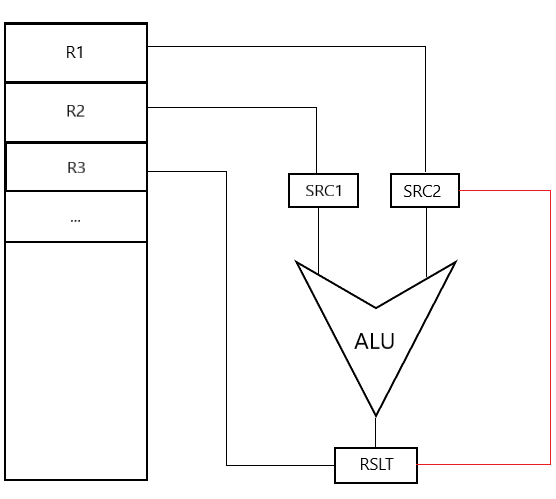
\includegraphics[width=0.6\textwidth]{operandus_elorehozas}
    \centering
    \caption{Az eredmény visszavezetése a forrás regiszterbe}
    \label{fig:operandus_elorehozas}
\end{figure}

\subsection{Lehívási adatfüggőség}
\paragraph{Probléma:} a regiszterekbe az operatív tárból (cache) töltjük be a szükséges adatokat, majd ezután a regiszterekből hívja le a végrehajtó egység (ALU).
A cache elérése viszont sok időt vesz igénybe.
Ennek látható az általános adatútja a \ref{fig:lehivas_elorehozas} ábrán, fekete vonallal jelölve.
\paragraph{Kezelés:} a folyamat gyorsítására extra hardvert alkalmazunk, amivel a cache-ből történő lehíváskor egyúttal a végrehajtó egységbe is betöltjük az adatot (piros vonal).
Így egy óraciklust megspórolhatunk.

\begin{figure}[H]
    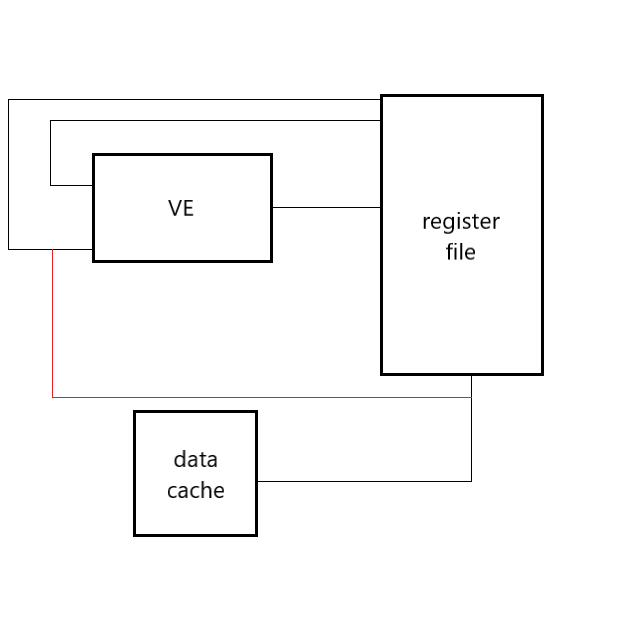
\includegraphics[width=0.6\textwidth]{lehivas_elorehozas}
    \centering
    \caption{A lehívott adat bevezetése a műveletvégző egységbe}
    \label{fig:lehivas_elorehozas}
\end{figure}

\subsection{WAR - Write After Read}

\paragraph{Probléma felvetés:} egy MUL utasítást egy ADD követ az alábbi módon:
\begin{lstlisting}[language=Ant]
    ;I1
    MUL r3,r2,1   ;r3 = r1 * r2
    ;I2
    ADD r2,r4,r5  ;r2 = r4 + r5
\end{lstlisting}
A szorzás (MUL) sokkal lassabb, mint az összeadás (ADD), ezért előfodulhat, hogy a párhuzamos
végrehajtás során I\textsubscript{2} hamarabb lefut, mint hogy I\textsubscript{1} betöltse a forrás operandust.
Mivel I\textsubscript{2} módosította I\textsubscript{1} bemeneti operandusát, a MUL utasítás hibás eredményt fog adni.
Következménye, hogy sérül a szekvenciális konzisztencia.
\paragraph{Megoldás:} r\textsubscript{2} tartalmát egy ideiglenes regiszterbe irányítjuk (pl. r\textsubscript{23}).
Ekkor az assmebly utasítások így néznek ki:
\begin{lstlisting}[language=Ant]
    ;I1
    MUL r3,r2,1   ;r3 = r1 * r2
    ;I2
    ADD r23,r4,r5 ;r23 = r4 + r5
\end{lstlisting}
Az r\textsubscript{23}$\,\to\,$r\textsubscript{2} hozzárendelést nyilvántartjuk, majd amikor a MUL utasítás végzett, visszaírjuk r\textsubscript{23} tartalmát r\textsubscript{2}-be.
Az átmeneti (átnevezési) regiszterek tulajdonságai:
\begin{itemize}
    \item új, önálló, de rejtett,
    \item saját címtartománnyal rendelkezik,
    \item a programozó számára traszparens,
    \item extra hardvernek számít.
\end{itemize}

\paragraph{Megjegyzés:} a regiszterkészletek csoportosítása:
\begin{itemize}
    \item architekturális: programozó használja,
    \item átnevezési: a vezérlés használja az álfüggőségek feloldására.
\end{itemize}

\subsection{WAW - Write After Write}
\paragraph{Probléma felvetés:} egy MUL utasítást egy ADD követ az alábbi módon:
\begin{lstlisting}[language=Ant]
    ;I1
    MUL r3,r2,1   ;r3 = r1 * r2
    ;I2
    ADD r3,r4,r5  ;r3 = r4 + r5
\end{lstlisting}
A szorzás (MUL) sokkal lassabb, mint az összeadás (ADD), ezért előfodulhat, hogy a párhuzamos
végrehajtás során I\textsubscript{1} később fut le, mint I\textsubscript{1}.
Mivel az eredményt ugyanabba a regiszterbe írják, ebben az esetben I\textsubscript{1} felülírja I\textsubscript{2} eredményét az r\textsubscript{3}-ban.
Ezzel sérül a szekvenciális konzisztencia.
\paragraph{Megoldás:} r\textsubscript{3} átirányítása egy átnevezési regiszterbe, az előbb leírt módon.

\subsection{Ciklusbeli függőség}

\paragraph{Probléma felvetés:}
egy ciklusban az előző iterációban kiszámolt adatot használunk fel, például:
\begin{algorithmic}
    \FOR{$i=2$ to $n$}
    \STATE X\textsubscript{i}$\leftarrow$A\textsubscript{i} * X\textsubscript{i-1} + B\textsubscript{i}
    \ENDFOR
\end{algorithmic}
\paragraph{Kezelés:} ez egy erős függőség, hardveresen nehezen feloldható. Megoldás az algoritmus áttervezése.

\section{Vezérlés függőségek}
Elágazások esetén léphetnek fel. Itt a statikus és dinamikus kezelésnek eltérő jelentése van, mint az adatfüggőségeknél. A statikus kezelés itt egy állandó, mindig alkalmazható eljárást jelent, míg a dinamikus kezelés az adott programtól függ.
\paragraph{Probléma felvetés:} az alábbi utasítássorozatban a feltétlen ugrás (JMP) egy SHL utasításra mutat:
\begin{lstlisting}[language=Ant]
    DIV
    MUL
    JMP ; SHL-re mutat
    ADD
    ...
    SHL
\end{lstlisting}
Ekkor a kritikus utasítások így követik egymást időben:
\begin{center}
    \begin{tabular}{ c | c | c | c | c | c | c }
            & t\textsubscript{1}   & t\textsubscript{2}   & t\textsubscript{3}   & t\textsubscript{4} & t\textsubscript{5} & t\textsubscript{6} \\
        \hline
        MUL & F\textsubscript{MUL} & D                    & E                    & W/B                &                    &                    \\
        \hline
        JMP &                      & F\textsubscript{JMP} & D                    & E                  & W/B                                     \\
        \hline
        ADD &                      &                      & F\textsubscript{ADD} & D                  & E                  & W/B
    \end{tabular}
\end{center}
A JMP utasítás az Execute fázisban állítja át a Program Countert, ezzel végzi el az ugrást.
A futószalag végrehajtás miatt azonban ekkorra már a következő utasítás, az ADD is lehívásra került, sőt, előfordulhat, hogy az azt követő utasítás is.
Ezek viszont fölösleges lépések. Ritkább esetekben a JMP-t követő utasítás be is fejeződhet, mire az ugrás végrehajtásra kerül, ami veszélyezteti az architekturális regisztertartalmakat.
\paragraph{Megoldás:} a probléma kezelése statikus, dinamikus, vagy spekulatív (branch prediction) módon történhet.
\paragraph{Kezelés utasítások átrendezésével (dinamikus):} compiler segítségével történő optimalizálás. A compiler megpróbálja átrendezni az utasítások sorrendjét.
Az előző kódrészlet optimalizált változata:
\begin{lstlisting}[language=Ant]
    JMP ; SHL-re mutat
    MUL
    DIV
    ADD
    ...
    SHL
\end{lstlisting}
Az optimalizálás utáni végrehajtási sorrend:
\begin{center}
    \begin{tabular}{ c | c | c | c | c | c | c | c }
            & t\textsubscript{1}   & t\textsubscript{2}   & t\textsubscript{3}   & t\textsubscript{4}   & t\textsubscript{5} & t\textsubscript{6} & t\textsubscript{7} \\
        \hline
        JMP & F\textsubscript{JMP} & D                    & E                    & W/B                  &                    &                                         \\
        \hline
        MUL &                      & F\textsubscript{MUL} & D                    & E                    & W/B                                                          \\
        \hline
        DIV &                      &                      & F\textsubscript{DIV} & D                    & E                  & W/B                                     \\
        \hline
        SHL &                      &                      &                      & F\textsubscript{SHL} & D                  & E                  & W/B
    \end{tabular}
\end{center}
A sorrend megváltoztatásával elértük, hogy amíg az ugrás végre nem hajtódik (t\textsubscript{3}), csak olyan utasításokat hívunk le, amiknek még az ugrás előtt kell lefutniuk.
Mire az ADD utasításhoz elérnénk, felülíródik a PC és a megfelelő utasítás hívódik le (SHL).
A módszer hátránya, hogy hatékonysága a futószalag fokozatok számának növelésével rohamosan csökken.
\paragraph{Kezelés NOP utasításokkal (statikus):} a JMP utasítás mögé egy vagy több NOP utasítás kerül be.
Ez a futószalag várakoztatását jelenti, amíg elő nem áll az ugráshoz szükséges PC. Ez az ún. ugrási buborék, nagysága $n-1$, ahol $n$ a futószalag fokozatok száma.

% Harmadik előadás

\chapter{Időbeli párhuzamosság: futószalag CPU-k}

\section{Bevezetés}
A futószalagos (pipeline) végrehajtás lényege, hogy egy utasítást több részre osztunk (általában fetch, decode, execute, writeback), majd ezeket a részeket külön, egymással párhuzamosan hajtjuk végre (\ref{fig:pipeline} ábra).
Az utasítások $n$ részre osztásával elméletileg a sebesség $n$-szeresére növekszik.
\begin{figure}[h]
    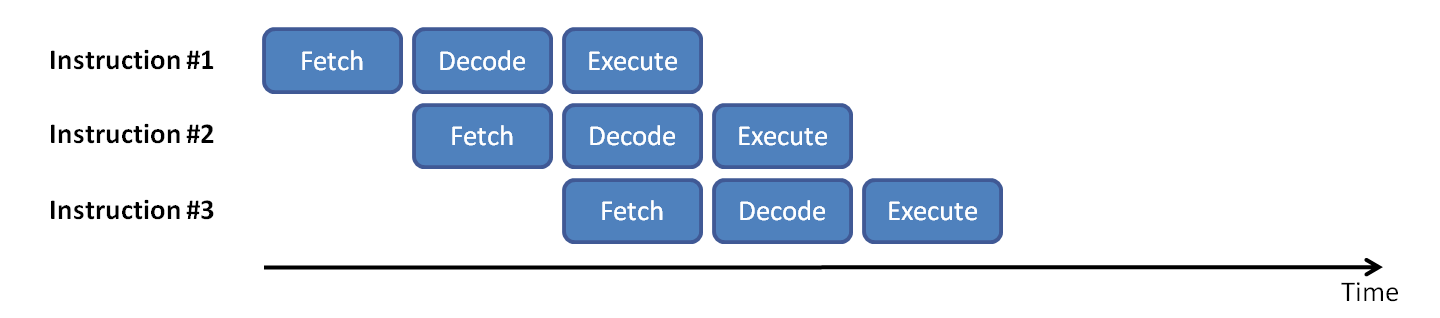
\includegraphics[width=0.6\textwidth]{pipeline}
    \centering
    \caption{Futószalagos végrehajtás}
    \label{fig:pipeline}
\end{figure}
\paragraph{A teljesítmény gátjai:} a gyakorlatban nem mindig valósul meg a fokozatok számának növekedésével arányos gyorsulás.
A végrehajtást a függőségek (adat, vezérlés, erőforrás) lassítják. A függőségek oka a sok párhuzamosan futó utasítás ($n+1$, ahol $n$ a fokozatszám).
\paragraph{A hatékonyság maximalizálása:}a tapasztalat szerint a hatékonyság kb. 15-30 fokozatú futószalag esetén maximalizálható, efölött a függőségek miatt már csökken a teljesítmény.
Ez az általános célú alkalmazásokra igaz, a mai általános processzorokban kb. 20 fokozat van. Speciális feladatokra (ahol kevés a függőség) használható superpipeline CPU, ami akár 200 fokozatú is lehet.

\section{Történeti áttekintés}
\begin{itemize}
    \item Intel 80486: 3 fokozat, de már külön lebegőpontos futószalag
    \item Intel Pentium (P5): 5 fokozat
    \item Intel Pentium III (P6): 11-17 fokozat
    \item Intel Pentium IV (Netburst): 20-31 fokozat
    \item Intel Core 2 (újratervezett P6, több mag): általában 14 fokozat
    \item Intel Core i: 16-20 fokozat
\end{itemize}

\section{Gyakorlati példa - az Intel Atom CPU}
Az Intel Atom processzor a 2000-es években jelent meg, 16 fokozatú futószalagot használ.
A processzor CISC (Complex Instruction Set Computing) architektúrájú, azaz egy utasításon belül nem csak a regiszterekből, hanem a memóriából, vagy a gyorsítótárból is képes adatot lehívni.
\paragraph{Az Intel Atom fokozatai:}
\begin{itemize}
    \item 1-3. fokozat: instruction fetch (IF)
    \item 4-6. fokozat: instruction decode (ID)
    \item 7-8. fokozat: instruction dispatch (SC - Switch Context, IS - Instruction Schedule)
    \item 9. fokozat: source operand read (IRF - Instruction Register File)
    \item 10-12. fokozat: data cache access, CISC architektúrához szükséges (AG - Address Generation, DC\textsubscript{1} - Data Cache 1, DC\textsubscript{2} - Data Cache 2)
    \item 13. fokozat: execute
    \item 14-15. fokozat: exception + multitask handling (FT\textsubscript{1} - Fault Tolerant 1, FT\textsubscript{2} - Fault Tolerant 2)
    \item 16. fokozat: commit, ez a visszaírás (W/B vagy DC\textsubscript{1})
\end{itemize}
\paragraph{Következmény:} ez egy tisztán futószalag elvű processzor, ami teljesítményben visszalépést jelentett a korábbi architektúrákhoz képest.
Előnye az alacsony fogyasztás, ezért főleg mobil eszközökbe használták az Atom CPU-kat.

\section{Futószalagos feldolgozás előfeltételei (2 fokozat esetén)}
Az ideális futószalag megvalósítható, ha
\begin{itemize}
    \item a számítógép 2 db egymástól független végrehajtó egységgel rendelkezik,
    \item az egyik fokozat kimenete a másik fokozat bemenete,
    \item mindkét fokozat végrehajtási ideje azonos,
    \item a fokozatok szinkronizáltak, órajelre kapják az inputot, és egyetlen óraciklus alatt elvégzik a feladatukat.
\end{itemize}
Ekkor $t=\frac{T}{2}$, ahol $T$ a szekvenciális végrehajtási idő és $t$ a futószalagos végrehajtási idő.

\section{Függőségek kezelése}
\begin{itemize}
    \item Operandus előrehozással:
    \begin{itemize}
        \item Minden architektúránál használják.
        \item Részletesen: \ref{fuggosegek}. fejezet.
    \end{itemize}
    \item Újrafeldolgozással:
    \begin{itemize}
        \item Leggyakrabban az execute fokozat egymás után többszöri végrehajtását jelenti.
        \item Pl. szorzásnál az ismétlődő összeadásokhoz használható.
        \item A futószalag feldolgozást lassítja, de összességében jobb teljesítményt biztosít.
    \end{itemize}
\end{itemize}

\section{Típusai}
\begin{enumerate}
    \item Előlehívás (overlapping)
    \item Vektor CPU-k (60-as évek)
    \item Teljes pipeline
\end{enumerate}

\subsection{Előlehívás}
A visszaírás során történik meg a következő utasítás lehívása:
\begin{center}
    \begin{tabular}{ c | c | c | c | c | c | c | c }
        & t\textsubscript{1} & t\textsubscript{2} & t\textsubscript{3} &t\textsubscript{4} & t\textsubscript{5} & t\textsubscript{6} & t\textsubscript{7} \\
        \hline
        I\textsubscript{1} & F & D & E & W/B \\
        \hline
        I\textsubscript{2} &   &   &   & F & D & E & W/B
    \end{tabular}
\end{center}
\paragraph{Előnyök:}
\begin{itemize}
    \item 4 óraciklus helyett csak 3 kell egy utasításhoz, így a teljesítmény 25\%-al nő, valamint
    \item nincsenek függőségek, mivel a forrás operandus beolvasásakor (t\textsubscript{5}) már megvan az előző utasítás eredménye (t\textsubscript{4}).
\end{itemize}
\paragraph{Hátrány:} nem túl nagy mértékű gyorsulás.

\subsection{Vektor CPU}
Csak az execute fokozat működött futószalagszerűen.

\subsection{Teljes pipeline}
A futószalagos feldolgozás kiterjesztése a teljes folyamatra:
\begin{center}
    \begin{tabular}{ c | c | c | c | c | c  }
        & t\textsubscript{1} & t\textsubscript{2} & t\textsubscript{3} &t\textsubscript{4} & t\textsubscript{5} \\
        \hline
        I\textsubscript{1} & F & D & E & W/B \\
        \hline
        I\textsubscript{2} &   &  F & D & E & W/B
    \end{tabular}
\end{center}

\section{Logikai futószalagok} \label{logikai_futoszalag}
Az eltérő utasítások eltérő felépítésű futószalagokat igényelnek, ezért egy processzor több futószalagot is tartalmaz.
A cél a funkcionális kialakítás. Példák különböző funkciókat ellátó futószalagokra:
\begin{itemize}
    \item aritmetikai: F, D, E, W/B
    \begin{itemize}
        \item fixpontos
        \begin{itemize}
            \item egyszerű: +, -, léptetés, ...
            \item összetett: *, /, ...
        \end{itemize}
        \item lebegőpontos
    \end{itemize}
    \item ugró (branch): F, E
    \item LOAD / STORE
\end{itemize}
\paragraph{Az utasítások értelmezése:} az utasításokat két szinten értelmezhetjük, pl. a fetch utasítás két szintje a következő:
\begin{enumerate}
    \item Fetch
    \item MAR $\leftarrow$ PC\\
    MDR $\leftarrow$ [MAR] \\
    IR $\leftarrow$ MDR \\
    PC $\leftarrow$ PC+1
\end{enumerate}

\section{Fizikai megvalósítás}
Alkalmazásuk alapján megkülönböztetünk univerzális és dedikált futószalagokat.
Az univerzális minden művelet elvégzésére alkalmas, míg a dedikált speciális műveletekre képes.
Hardveres szempontból az univerzális futószalag előnytelen, mivel sok tranzisztorra van szükség, a kialakítása bonyolult és drága, ráadásul a végrehajtás lassú.
Ezért általában a \ref{logikai_futoszalag}. részben leírt dedikált (egy adott funciót ellátó) futószalagokat építenek a processzorokba.
Az eredmény kevesebb logikai kapu, így gyorsul a végrehajtás (a bemenettől a kimenetig gyorsabban átérnek az elektronok).
\paragraph{Megjegyzés:} a futószalag sebességét általában a leglassabb fokozat sebessége határozza meg, tehát a tervezési cél a megközelítőleg azonos sebességű fokozatok létrehozása.
\paragraph{Fokozatok kialakítása:} a fokozatok előtt előválasztó (puffer) regiszterek vannak. Ezek a felhasználó számára láthatatlanok, az adat először ezekbe töltődik be.
Ezekből a regiszterekből kerül aztán a végrehajtó egységbe az adat, majd az utasítás elvégzése után szintén puffer regiszterekbe kerül a kimenet.
A puffer regiszterek szükségesek, mivel a gyakorlatban egy fokozat nem mindig végez egy óraciklus alatt.
Az ebből adódó várakozás során ezekben a regiszterekben tárolódik az adat.
Ennek a kialakítása látható a \ref{fig:fokozat}. ábrán. A későbbiekben a végrehajtó egységekből egymás mellé többet is helyeztek, így megvalósítva a térbeli párhuzamosságot (\ref{fig:fokozat_parhuzamos}. ábra).
\begin{figure}[h]
    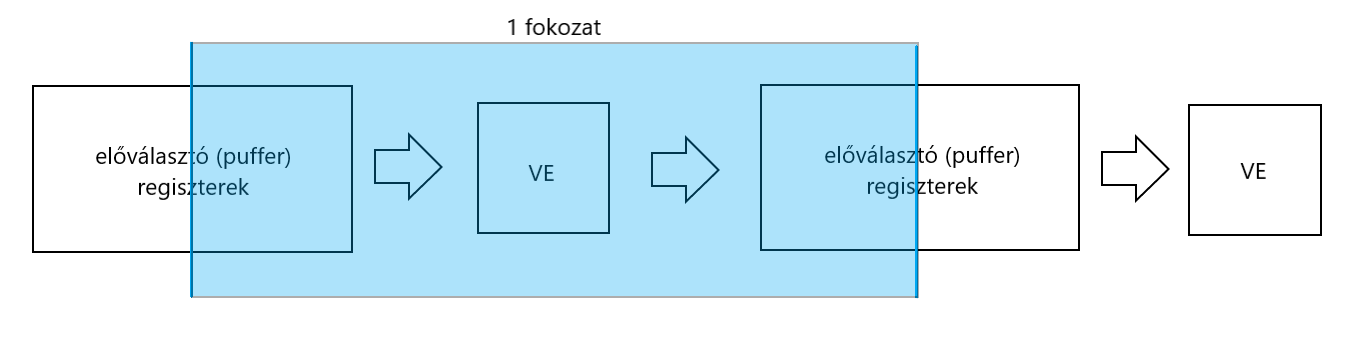
\includegraphics[width=0.6\textwidth]{fokozat}
    \centering
    \caption{A fokozatok felépítése}
    \label{fig:fokozat}
\end{figure}
\begin{figure}[h]
    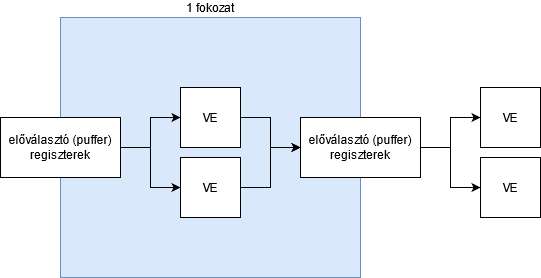
\includegraphics[width=0.6\textwidth]{fokozat_parhuzamos}
    \centering
    \caption{A végrehajtó egységek párhuzamosítása}
    \label{fig:fokozat_parhuzamos}
\end{figure}

\subsection{Példa: a PowerPC 604}
A PowerPC 604-es processzorban egymással párhuzamosan több dedikált futószalag is működött (\ref{fig:powerpc604} ábra).
A fetch és decode fokozatok minden óraciklusra lehívtak egy utasítást, és a megfelelő futószalagba töltötték.
Így a CPU képes volt egymással párhuzamosan több utasítást is végrehajtani (akár 4-et is).
Mivel előfordulhatott, hogy a később lehívott és betöltött utasítás végzett hamarabb (pl. elsőként egy FP, másodikként egy FX utasítás $\rightarrow$ FX hamarabb végez), szükséges volt egy konzisztencia fokozat (CO) bevezetése.
Az utasítások címkézésre kerültek, a sorrendet a CO biztosította.
A párhuzamosság miatt szükség volt a fokozatok közötti várakoztatásra, ez az interlock funkció.
\paragraph{Megjegyzés:} az Intel 80486 és az első Pentium csak 2 utasítás futószalaggal rendelkezett. A mai Core i architectúrák magonkánt általában 6-8 futószalagot alkalmaznak.
\label{powerpc604}
\begin{figure}[H]
    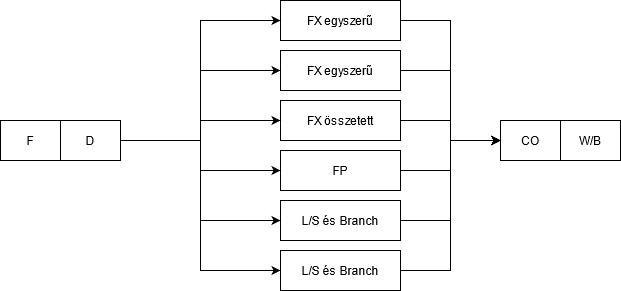
\includegraphics[width=0.6\textwidth]{powerpc604}
    \centering
    \caption{A PowerPC 604 futószalagja}
    \label{fig:powerpc604}
\end{figure}

\section{RISC és CISC architektúrák}
Az utasításkészlet (tervezési stratégia) alapján kétféle architektúrát különböztetünk meg:
\begin{itemize}
    \item RISC: Reduced Instruction Set Computing - csökkentett utasításkészletű architektúra és
    \item CISC: Complex Instruction Set Computing - bővített utasításkészletű architektúra.
\end{itemize}
Mindkettő használatban van napjainkban.
\subsection{Történeti áttekintés}
Az első CPU-k kevés utasítással rendelkeztek (RISC), majd a 70-es években az egyre több funkció és bonyolultabb utasítások miatt ez a szám növekedett (CISC).
A 80-as években rájöttek, hogy a sok utasítás ugyan megkönnyíti a programozást, de a címzés bonyolultsága miatt káros hatással van a teljesítményre.
Ez vezetett a RISC architektúrák újbóli megjelenéséhez.

\subsection{RISC}
\paragraph{Példa:} a mobil eszközök ARM (Advanced RISC Machine) processzorai RISC architektúrájúak.
\paragraph{Tulajdonságai:}
\begin{itemize}
    \item Kis számú (50-150) utasítással rendelkezik $\rightarrow$ címzési módok egyszerűsödése.
    \item Nincs olyan utasítás, ami a LOAD/STORE-t aritmetikával kombinálja (nem lehet egyszerre betölteni az adatot és végrehajtani a műveletet).
    \item Minden műveletvégző utasítás regisztereket használ $\rightarrow$ memóriából vagy gyorsítótárból nem lehet dolgozni.
    \item Memória vagy cache elérés csak LOAD/STORE utasításokkal történhet.
    \item Nagy számú regiszterkészlet (mivel minden művelethez regiszterekre van szükség).
    \item Általában 3 operandusos utasítások $\rightarrow$ az eredmény nem írja felül a bemeneti regisztert, hanem külön regiszterbe kerül.
    \item Minden utasítás hossza egyforma (pl. 128 bit) $\rightarrow$ könnyebb a futószalagos feldolgozás.
    \item A fordítóprogramok bonyolultabbak a kevés utasítás miatt.
    \item Általában huzalozott (hardveres) az utasítás feldolgozás (decode).
    \item Utasítás végrehajtás általában egy óraciklust vesz igénybe (cél az egyforma ciklusidő).
\end{itemize}
\paragraph{Előnye:} általában gyorsabb végrehajtás a CISC architektúrákhoz képest.
\paragraph{Hátránya:} a bonyolultabb feladatokat instrukció szekvenciákkal kell megoldani.
Ez a fordításnál okoz problémát, növelheti a program méretét.

\subsection{CISC}
\paragraph{Példa:} a 80-as években elterjedt Intel 80386-os egy tisztán CISC architektúra.
\paragraph{Tulajdonságai:}
\begin{itemize}
    \item Nagy számú utasításkészlet (több száz).
    \item A sok utasítás nagy belső mikroprogramtárat igényel.
    \item Sokféle címzési mód (tartalmaz típus címzési módot is) és sokféle utasítás.
    \item Változó méretű (akár összetett) utasítások $\rightarrow$ a dekódolónak nem csak dekódolni kell az utasítást, hanem azonosítani is az utasítás végét (tudnia kell, hogy hol fejeződik be). Ezt hívják utasítás határra illesztésnek, plusz hardvert és időt igényel.
    \item Közvetlen memória elérés lehetsége $\rightarrow$ a második operandus lehet memória vagy cache cím is.
    \item Két operandusos utasítások $\rightarrow$ az első operandus felülíródik az eredménnyel.
    \item Az előző kettőből következik, hogy az első operandus nem lehet memória/cache cím, mivel az eredmény memóriába írása nagyon lelassítaná a működést.
    \item Az utasítások feldolgozása több ciklusidő lehet $\rightarrow$ bonyolultabb feldolgozás.
    \item Egyszerűbb a gépi kódú programozás a sokféle utasítás miatt (egyszerűbb fordítóprogramok).
    \item Egy utasításban több elemi műveletet is végre tud hajtani.
    \item Az utasítások folyamatosan bővültek, így a régi programokkal visszafelé kompatibilis maradt.
    \item A futószalag fokozatok között sebesség különbség lehet $\rightarrow$ feloldására interlock funkciót használnak (részletesen: \ref{powerpc604}).
    \item Általában a memória elérés miatt +2 fokozat szükséges a RISC-hez képest (AG - címszámítás és cache elérés).
\end{itemize}
\paragraph{Előnyei:} kompatibilitás a régi programokkal, egyszerűbb compilerek.
\paragraph{Hátránya:} bonyolultabb, lassabb végrehajtás.

\subsection{Hibrid CISC}
\paragraph{Példa:} az x86-os architektúra ISA-t (Instruction Set Architecture) használ, ami egy hibrid CISC architektúra.
\paragraph{Tapasztalat:} megfigyelték, hogy a CISC processzorok az idő 80\%-ában az utasítások mindössze kb. 20\%-át használják.
\paragraph{Optimalizálás:} a feldolgozás gyorsítása érdekében kialakítottak a CISC architektúrán belül egy RISC magot.
Ez a megoldás minden mai (Core i) architektúrában megjelenik.

\subsection{Hibrid RISC}
A mai ARM processzorok sem tisztán RISC architektúrák, hanem CISC jellegű utasításokkal vannak kibővítve (pl. az ARM Thumb, ami egy tömörített utasításkészlet).

\section{Következmények}
A futószalagos feldolgozás következményei:
\begin{itemize}
    \item Jelentősen felgyorsult az utasítások lehívása és az operandusok betöltése.
    \item Amíg a processzorok feldolgozási sebessége jelentősen nőtt, a memória sebessége kevésbé (ez a jelenség a sebességolló) $\rightarrow$ cache bevezetése (IBM - 1968, Intel - 80-as évek). A cache előnye, hogy a gyakran használt operandusok gyorsan elérhetők.
    \item Maximális végrehajtási sebesség: 1 utasítás / ciklus (további növekedés kibocsájtási párhuzamossággal vagy utasításon belüli párhuzamossággal lehetséges).
    \item A vezérlés átadási utasítások kifinomult technikája szükséges (függőségek miatt).
    \item Az elágazás kezelés bonyolódik.
\end{itemize}

\subsection{Elágazások kezelése}
\subsubsection{Korai RISC gépek}
Kezelés ugrási buborékkal.
\subsubsection{Korai CISC gépek}
A dekódoló fokozatba építették a címszámító és a logikai komparáló egységet, így a dekódolási ciklus végére előáll az ugrási cím.
\subsubsection{Későbbi CISC gépek (futószalag CPU-k és első generációs szuperskalár architektúrák)}
Kezelés fix előrejelzéssel, pl. mindig ugrik.
Ezzel a megoldással az ugrási cím előre kiszámításra kerül és megkezdődik az ugrási címen lévő utasítások lehívása.
Ha mégse kell ugrani, az utasításokat visszatörli és az eredeti helyen folytatódik a végrehajtás.
Előnye, hogy kiküszübölte az ugrási buborékot, növekszik a teljesítmény.
Korlátja, hogy ha nagy látenciával rendelkező műveletet kellett végrehajtani az ugrási feltételben, az blokkolta a kibocsájtást.
Ilyen megoldást használ például az Intel 80486-os CPU.
\subsubsection{Második generációs szuperskalár architektúrák}
A CPU a dekódolási folyamatok egy részét már akkor elvégzi, amikor az utasításokat az L1 cache-be írja.
Az előre elvégzett feladatok:
\begin{itemize}
    \item utasítás típusazonosítás
    \item ugrások felismerése
    \item utasításhossz meghatározása (szükséges, mivel CISC-nél változó az utasításhossz)
    \item spekulatív elágazásbecslés
    \begin{itemize}
        \item regiszterátnevezéssel
        \item átrendező puffer (Intel: ROB - ReOrder Buffer)
    \end{itemize}
\end{itemize}

\section{Összegzés}
A fejezetben felsorolt módszerekkel elérték a futószalag elvű processzorok teljesítményének korlátait.
A további gyorsítás érdekében párhuzamos kibocsájtást kellett alkalmazni, így jöttek létre a szuperskalár processzorok.
% Második előadás

\chapter{Nagy teljesítményű, két foglalatos szerver processzorok fejlődése}

\section{Szerver platformok osztályozása}
A szerver rendszerek feloszthatók egy processzoros (UP) és több processzoros platformokra.
A több processzoros platformok feloszthatók két foglalatos (2S/DP), négy vagy nyolc foglalatos (4S, 8S) és nyolcnál több foglalatos rendszerekre.
A piac nagy részét a két processzoros szerverek teszik ki (kb. 80\%), ezért részletesebben ezekkel foglalkozunk.

\section{Méret, tranzisztorok}
A 2S szerver processzorok nagy méretűek, sok tranzisztort tartalmaznak.
A 2000-es évek közepén a Pentium 4 szerver processzorok még viszonylag kevés tranzisztorból álltak (125 millió), ezért elég volt kb 1 cm\textsuperscript{2}-es lapka.
A magok számának növekedésével egyre több tranzisztor kellett, a Skylake (2017) processzoroknál már 8 milliárd.
Még újabb CPU-knál nincs információ.
Ezzel együtt a lapkaméret is tovább nőtt, a mai lapkáknál 8 cm\textsuperscript{2} körüli.

Mivel a lapkák gyártása nagyon komplex, nagyobb méretű lapkáknál több hiba előfordulhat, ezért alacsonyabb lesz a kihozatali arány.
A lapkák méretét így a gazdasági hatékonyság is meghatározza.

\section{Fogyasztás}
A HEDT processzoroknál is nagyobb fogyasztással kell számolni a szerver processzoroknál, 130-tól 200 W felettig mennek.

\section{Lábak száma}
A szerver processzorok sok lábbal kapcsolódnak a foglalatokhoz, amik precíz gyártást igényelnek.

\section{Magok száma}
A szerver alkalmazások általában jól párhuzamosíthatók, így a processzorok a lehető legtöbb magot implementálják.
A Pentium 4 szerver processzoránál még csak 1 mag volt, de később 28-ig növekedett a magok száma.

\section{Intel Cascade Lake 9200-AP}
Ez a 2x28, azaz 56 magos processzor az Intel válasza volt az AMD 64 magos EPYC Rome processzoraira.
Az AMD 2017-ben adta ki ezt a processzort, ami valós konkurenciát állított az Intelnek, ami 2015 környékén még nagyrészt egyeduralkodó volt a szervereknél.
Ezért az Intel két 28 magos lapkát tett egy foglalatba, és BGA (Ball Grid Array) tokozással látta el, ami forrasztásra készült.
A forrasztás miatt nem voltak külön megvásárolhatók, csak OEM-ek kapták meg.

A két lapka egybecsomagolása miatt egy két foglalatos rendszer gyakorlatilag 4 processzort jelent.

\section{Magszámok és tranzisztorok növekedése}
A kétfoglalatos szerver CPU-k esetében kb 2 évente duplázódott a magok száma (\ref{fig:core}. ábra).

\begin{figure}[H]
    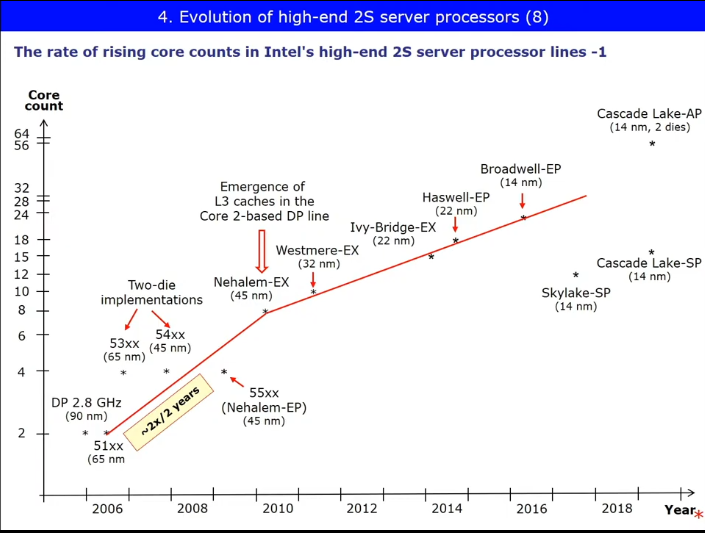
\includegraphics[width=0.8\textwidth]{core}
    \centering
    \caption{Intel 2S szerver processzorok magszámának fejlődése}
    \label{fig:core}
\end{figure}

Ez összhangban van a Moore-szabállyal, ami szerint a tranzisztorok száma két évente duplázódik.
Az utóbbi években viszont lelassult a fejlődés, már csak négy évente duplázódott a magok száma.
Ennek egyik oka az L3 cache megjelenése, ami elfoglalja a lapka jelentős részét, mivel nagyon sok tranzisztor kell a működéséhez.
A technológi változása miatt a Moore törvénnyel ellentétben az Intel már csak 4 évente tudta duplázni a tranzisztorok számát (\ref{fig:transistor}. ábra).
Ennek az oka, hogy a sok tranzisztor disszipációját kezelni kell, ami korlátozza a fejlődést.

\begin{figure}[H]
    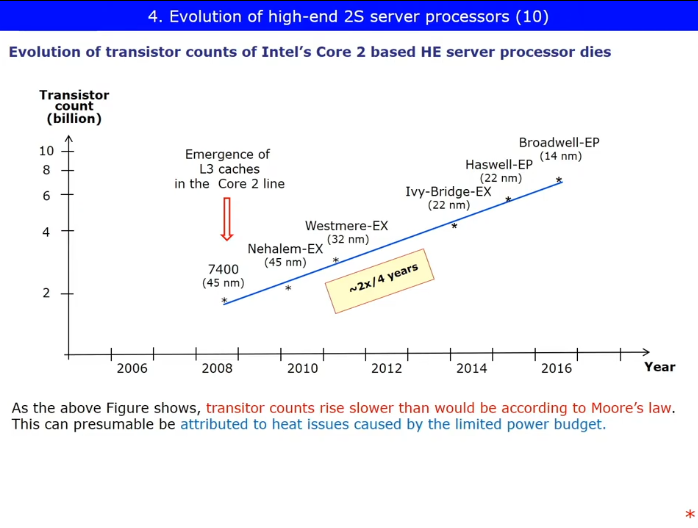
\includegraphics[width=0.8\textwidth]{transistor}
    \centering
    \caption{Intel 2S szerver processzorok tranzisztorszámának fejlődése}
    \label{fig:transistor}
\end{figure}

\subsection{Kivételek}
Néhány processzor az ábrán nem illik a fejlődési görbére, ezek az AMD konkurenciára adott válaszoknak köszönhetők.

\section{Memória sebességek fejlődése}
A memória sebességeknél adatátviteli rátával jellemezzük őket, mivel a frekvencia nem azonos az átviteli sebességgel a DDR (Double Data Rate) memóriák esetében.

\begin{figure}[H]
    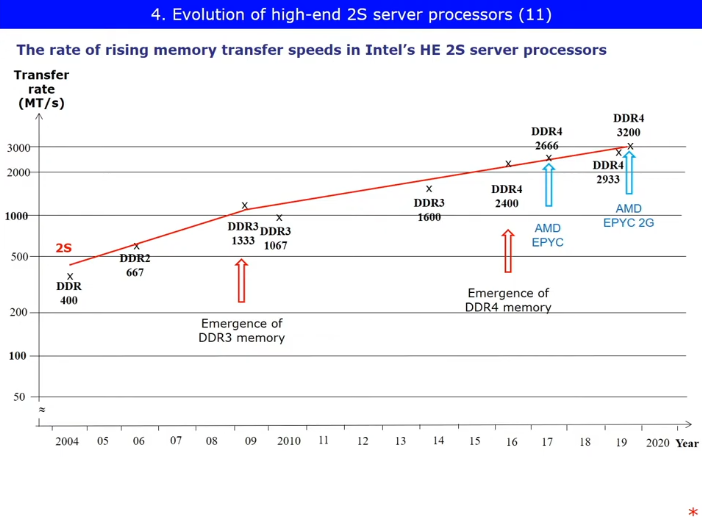
\includegraphics[width=0.8\textwidth]{mem}
    \centering
    \caption{Memória sebességek fejlődése}
    \label{fig:mem}
\end{figure}

A \ref{mem}. ábrán látható, hogy a DDR és DDR2-es memóriák gyorsabban fejlődtek, mint a DDR3 és DDR4 memóriák.
Az első szakaszban egy duplázódáshoz 4 év kellett, DDR3 óta pedig már 8.
Ennek oka a DDR3-as memóriák jóval komplexebb felépítése, ami lassította a fejlődést.
A magok száma tehát gyorsabban növekedett, mint a memóriák sebessége, ami konfliktusforrás.

Szerverek esetében elvárás, hogy az egymástól függetlenül működő magokat azonos memória sávszélességgel kell ellátni.
Tehát a sávszélességet lineárisan skálázni kell a magszámmal együtt.
A foglalatonkénti sávszélesség kiszámítása:
\begin{equation}
    BW/core = n_M*w*T_M/n_C
\end{equation}
ahol:
\begin{itemize}
    \item n\textsubscript{M}: memória csatornák száma
    \item w: memória csatorna szélessége (pl. 8 byte)
    \item T\textsubscript{M}: memória átviteli rátája (pl. 2.4 GT/s)
    \item n\textsubscript{C}: magok száma
\end{itemize}

Probléma, hogy a transzfer ráta lassabban nő, mint a magok száma, tehát $T_m/n_C$ folyamatosan csökken.
Megoldás a memória csatornák számának növelése.
Ez azonban elég komplex feladat.

A magonkénti memória sávszélességnél referenciának tekinthető a Pentium 4 DP rendszer, a fejlesztési cél ehhez az értékhez tartani.

% Hetedik előadás

\chapter{Lebegőpontos és BCD számok}

\section{Bevezetés}
A lebegőpontos számok szükségesek, mivel:
\begin{itemize}
    \item a fixpontos számok értelmezési tartománya viszonylag kicsi
    \item fixpontos számoknál a pontosság is viszonylag kicsi
\end{itemize}

A lebegőpontos számokat 1985-ben szabványosították (IEE754).
Formájuk: $M*r^k$, ahol M a mantissza, r a radix és k a karakterisztika.
Fontos, hogy r alapja megegyezzen az M számrendszerének alapjával.

\section{Ábrázolás}
A lebegőpontos számok ábrázolása normalizált formátumban történik, tehát a tizedes (kettes számrendszernél kettedes) pont után következik az első értékes számjegy.
Példa: $0,1011*2^k$.

\section{A mantissza lehetséges értékei}
Ezzel a mantissza értéke fix intervallumba kerül, pl. 10-es számrendszernél $0,1 <= M < 1$.
Ugyanez általánosan megfogalmazva: $1/r <= M < 1$.

\section{Értelmezési tartomány}
A lebegőpontos számok értelmezési tartománya függ:
\begin{itemize}
    \item a karakterisztika számára rendelkezésre álló bitek számától
    \item a radixtól
\end{itemize}

\section{Pontosság}
Példa: $0,3014*10^6$.
Ekkor ha a mantisszára 3 bitet allokálunk, elveszítjük a 4-es számjegyet, csökken a pontosság.
A pontosság tehát függ a mantissza hosszától (rendelkezésre álló bitek számától).

\section{Alulcsordulás és túlcsordulás}
Az értelmezési tartományon kívül eső értékeket nem tudjuk ábrázolni, így ott túlcsordulás keletkezik.
Mivel a mantisszának 0,1-nél nagyobb vagy egyenlőnek kell lennie, ezért a nullát sem tudjuk ábrázolni, alulcsordulás keletkezik.
Az alul- és túlcsordulási régiók nagysága elsősorban a karakterisztikára allokált bitektől függ.
\begin{figure}[H]
    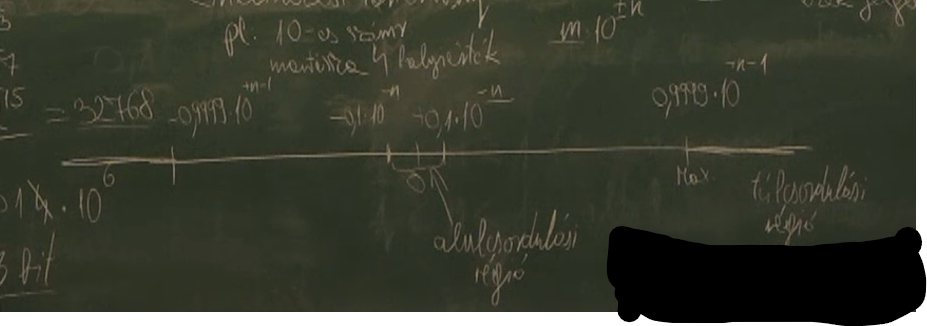
\includegraphics[width=0.8\textwidth]{csord}
    \centering
    \caption{Alul- és túlcsordulási régiók}
    \label{fig:csord}
\end{figure}

Az architektúrának biztosítania kell a túlcsordulás felismerését, jelzését és kezelését.

Az architektúra lehetőségei túlcsordulás esetén:
\begin{itemize}
    \item kijelzi a túlcsordulást és beállítja a legnagyobb megengedett értéket
    \item kijelzi a túlcsordulást és előjeles végtelent jelez ki
\end{itemize}
Alulcsordulás esetén:
\begin{itemize}
    \item kijelzi az alulcsordulást és nullára konvertál
    \item kijelzi az alulcsordulást denormalizált számot jelzi ki
\end{itemize}
A kijezést flagek segítségével teszi.

A szabvány előírja, hogy ha a mantissza nulla, a karakterisztikának is nullának kell lennie.

\section{Pontosság növelése}
Probléma, hogy a tízes számrendszerben pontosan megadható számok egy része kettes számrendszerben végtelen tizedes törtként ábrázolható (pl. 0.3).
A pontosság növelésére alkalmazott módszerek:
\begin{itemize}
    \item rejtett bit használata: a mantissza tört utáni részénél az első számjegy (bit) mindig 1, így nincs információtartalma. Ezért azt nem tároljuk, így egy bittel pontosabb számot tudunk tárolni.
    \item őrző bitek: a szabvány elvárása, hogy a pontatlanság kisebb legyen, mint a normalizált eredmény legkisebb számjegye. Probléma, hogy normalizáláskor értékes biteket veszíthetünk el, ezért a CPU-n belül a regiszterek több biten tárolják a mantisszát. Általában +3-15 bit. Ezek az őrző bitek, amik a memóriában tárolás során nem jelennek meg. Az őrző bitek felhasználása:
    \begin{itemize}
        \item a rejtett bit balra léptetésekor értékes bitet tudunk beléptetni
        \item tárolási formátum kérésekor kerekített értéket tárolhatunk
        \item normalizáláskor értékes biteket tudunk felhasználni
    \end{itemize}
\end{itemize}

\section{Lebegőpontos műveletvégzés jellemzői}
\begin{itemize}
    \item kódolás: mantissza kódolása 2-es komplemens, karakterisztika kódolása többletes kódolással. Ennek oka, hogy a többletes kód kialakítása gyorsabb, de elsősorban csak összeadás és kivonás elvégzésére alkalmas. Szorzást, osztást egyszerűbb kettes komplemenssel kódolt számokon könnyebb.
\end{itemize}

\section{IEEE 754 további jellemzői}
A szabvány fő célja a kompatibilitás megteremtése különböző CPU-k között.
A hardvernek és a szoftvernek együtt kell biztosítania a szabványnak való megfelelést.

A szabvány legfontosabb fejezetei:
\begin{itemize}
    \item adattípus
    \item formátumok
    \begin{itemize}
        \item szabványos (háttértáron tárolás)
        \begin{itemize}
            \item egyszeres pontosságú (32 bit)
            \item kétszeres pontosságú (64 bit)
        \end{itemize}
        \item kiterjesztett (CPU-n belül)
        \begin{itemize}
            \item egyszeres pontosságú (32 bit)
            \item kétszeres pontosságú (64 bit)
        \end{itemize}
    \end{itemize}
    \item műveletek
    \item kerekítések
    \item kivételek kezelése
\end{itemize}

A szabvány által meghatározott műveletek:
\begin{itemize}
    \item négy aritmetikai művelet
    \item maradékképzés
    \item gyökvonás
    \item bináris-decimális konverzió
    \item értelmezett a végtelennel való műveletvégzés
    \item kerekítések
    \begin{itemize}
        \item legközelebbire kerekítés
        \item nullára kerekítés (őrző bitek levágása)
        \item kerekítés pozitív végtelen felé
        \item kerekítés negatív végtelen felé
    \end{itemize}
\end{itemize}

A kivételek felbukkanása általában megszakítást eredményez.
Kivételek lehetnek pl. overflow, underflow, nullával osztás, gyökvonás negatív számból.

Először a lebegőpontos egységek koprocesszorokban voltak, később az Intel 80486 CPU-nál már a processzorba volt integrálva.

\section{Műveletek megvalósítása}

\begin{itemize}
    \item A+B: azonos hatványra hozás és összeadás
    \item A*B: A és B mantisszájának szorzása és a karakterisztikák összeadása
\end{itemize}
A szorzásnál fontos, hogy a két művelet párhuzamosan elvégezhető, így növelhető a sebesség.
Ennek a megvalósítása dedikált FP műveletvégzővel történik: egy adatbuszon keresztül a mantissza a mantissza egységbe, a karakterisztika pedig a karakterisztika egységbe kerül, a végeredményt pedig a vezérlő rakja össze.

\section{BCD számábrázolás}
Megjelenésének fő oka a fixpontos és a lebegőpontos számok pontatlansága.
Elsősorban adminisztratív és tudományos alkalmazásoknál használják (pl. számológépek).
A lebegőpontos konvertálás lehet pontatlan, de a kódolás pontos megfeleltetés, nincs kerekítés.

BCD kódolásnál minden számjegyet 4 biten ábrázolunk.
Mivel 4 bit 16 féle értéket vehet fel, keletkezik 6 darab érvénytelen tetrád, ami nincs használatban BCD kódolásnál.

\subsection{Ábrázolási formátumok}
\begin{itemize}
    \item zónázott: 1 byte = 1 számjegy, minden tetrádot megelőz 4 zóna bit
    \item pakolt: 1 byte = 2 számjegy (pl. Intel)
\end{itemize}

\subsection{Műveletvégzés logikai szinten}
Példa: 8+7=15.
BCD kódolva ez 1000+0111=1111, ami egy érvénytelen tetrádot eredményez, így 10-et ki kell vonni belőle (azaz hozzáadunk -10-et).
Kettes komplemens esetben 1010 invertálva 0101, majd hozzáadva egyet 0110.
Ezzel előáll az 5 mint eredmény.

\subsection{Műveletvégzés áramköri szinten}
A megvalósításhoz szükség van 4 db teljes összeadóra.
Az áramkörnek el kell végeznie az érvénytelen tetrádok kezelését is.
Az előző példánál az áramkör működése:
\begin{figure}[H]
    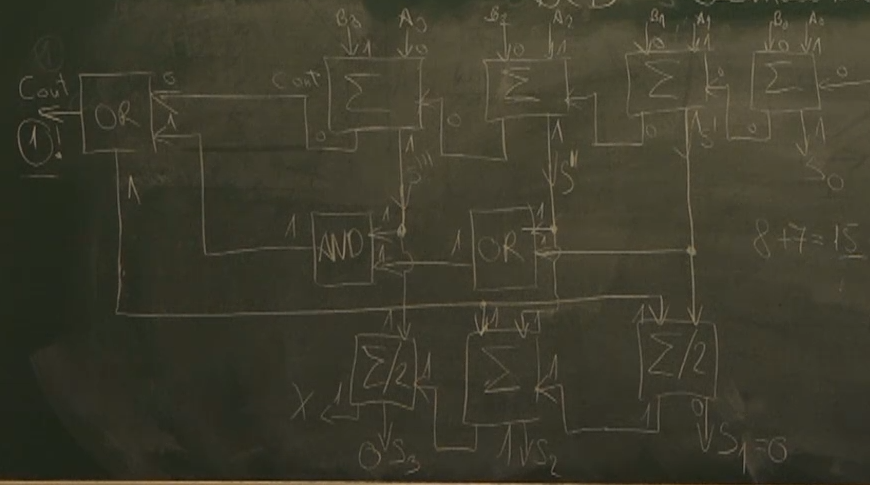
\includegraphics[width=0.8\textwidth]{bcd}
    \centering
    \caption{BCD összeadó áramkör}
    \label{fig:bcd}
\end{figure}

\subsection{Összegzés}
A BCD kódolás előnye tehát, hogy teljesen pontos, viszont jelentősen több helyet foglal, mint a lebegőpontos számok, valamint lassabb a végrehajtás is sok esetben.
A BASIC programnyelv ezt használja.

\section{Az ALU egyéb műveletei}
Az aritmetikai műveleteken kívül egyéb műveleteket is ellát az ALU, ezek általában egyszerűbb áramköröl segítségével megoldhatók.
\begin{itemize}
    \item Boole műveletek (mind a 16 fajta) pl.:
    \begin{itemize}
        \item AND
        \item NOR
        \item XOR
    \end{itemize}
    \item léptetés
    \item invertálás
    \item komparálás (feltételes ugrás)
    \item LOAD/STORE címszámítás - valós időben címet generál a MAR számára
    \item karakteres műveletek
\end{itemize}
% 8. előadás második fele, 9. előadás első fele

\chapter{Az Intel Netburst architektúra}

\section{Bevezetés}
A második generációs szuperskalárok fejlesztése során a 90-es évek második felében elérték az architektúra teljesítménybeli korlátait.
A hatékonyság növelésének extenzív forrásai kimerültek.
A sebesség további fokozásához a következő módszerekkel keresték a megoldást:
\begin{itemize}
    \item új architektúrák, pl. VLIW (ld. \ref{vliw}. fejezet)
    \item párhuzamosság egyéb forrásai (szál vagy folyamat szintű párhuzamosság)
    \item frekvencia erőteljes növelése
\end{itemize}
Az Intelnél a frekvencia erőteljes növelésével próbálkoztak, de az akkori legfejlettebb architektúrájuk, a P6 (Pentium III alapja) nem volt alkalmas 1333 MHz fölötti működésre.
A fejlesztés során a 10 GHz elérését tűzték ki célul, így új architektúra kellett.
Ez lett a Netburst architektúra, amire a Pentium IV processzorcsalád épült.
Az architektúra nem jelentette a második, illetve harmadik generációs szuperskalárok gyökeres újratervezését, a célkitűzés mindössze a magasabb frekvenciás működés volt.

\section{A frekvencia növelése}
A frekvencia növeléséhez a következő változtatásokat vezették be:
\begin{itemize}
    \item Gyártási csíkszélesség csökkentése (180 nm $\rightarrow$ 65 nm), általában egy lépésben 0.7-szeresére csökkentik (így fele akkora helyen fér el ugyanannyi tranzisztor, mint a korábbi technológiánál, tehát a tranzisztorok száma megduplázható $\rightarrow$ Moore-törvény).
    \item Futószalag fokozatok hosszának csökkentése (ennek egyik módja a fokozatok kisebb részekre bontása, viszont ekkor a fokozatok száma növekszik, nő a párhuzamosan végrehajtott utasítások száma és a függőségek száma is $\rightarrow$ csökkenhet a hatékonyság).
\end{itemize}

\section{Jellemzői}
\begin{itemize}
    \item CISC architektúra (1-17 byte hosszú utasítások)
    \item belső RISC mag
    \item hosszabb futószalagok (több függőség, de magasabb frekvencia)
\end{itemize}

\section{Újdonságok}

\subsection{Execution Trace Cache}
Az Execution Trace Cache az L1 utasítás cache-nek felel meg, de CISC helyett már dekódolt RISC utasításokat tartalmaz a végrehajtásuk feltételezett sorrendjében.

\subsection{Hyper futószalag}
A Hyper futószalag lényege, hogy a dekódoló fokozat nincs benne.
A dekódolás futószalagon kívül történik, azért, hogy az L1 cache-ben (Execution Trace Cache) már dekódolt és átalakított utasítások szerepelhessenek.
Oka, hogy a CISC utasítások átalakítása lassú, akadályozta volna a nagy frekvenciás végrehajtást, ezért külön került a futószalagtól.
Újdonság még, hogy a korábbi 10-15 fokozathoz képest 20-31 fokozatot tartalmazott.
Ennek hátránya, hogy hibás becslés esetén nagyobb a büntetés, több fokozatot kell törölni a futószalagból $\rightarrow$ fajlagos teljesítmény csökkenés.

\subsection{Enhanced Branch Prediction}
Ez egy továbbfejlesztett elágazásbecslő logika, 94-97 \%-os hatékonysággal (PIII-hoz képest kb. 33 \%-al csökkent a hibás becslések száma).

\subsection{Quad Data Rate Bus}
A Quad Data Rate Bus egy belső rendszerbusz, gyorsítja az adatelérést az L1 és L2 gyorsítótárak felé.
A buszfrekvencia négyszeresén továbbítja az adatokat (a külső rendszerbusz sebességét nem lehetett növelni, mivel a memória nem gyosult jelentősen). Ennek eléréséhez kettő órajel generátort alkalmaz, 90\textdegree-os fáziseltolással, valamint a felfutó és lefutó élen is történik adattovábbítás.
Így óraciklusonként négy adattovábbítás történik.
Ezt a működést mutatja be a \ref{fig:qdrb}. ábra.
\begin{figure}[h]
    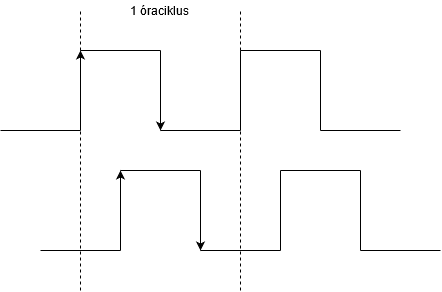
\includegraphics[width=0.6\textwidth]{qdrb}
    \centering
    \caption{A Quad Data Rate Bus kettős órajele}
    \label{fig:qdrb}
\end{figure}

\subsection{Rapid Execution Engine}
A Rapid Execution Engine az egyszerű FX műveletek gyors végrehajtására szolgáló végrehajtó egység.
Az órajel felfutó és lefutó élére is képes műveletvégzésre, így a végrehajtási idő akár egy fél ciklusra is csökkenhet.
A gyorsaság érdekében kevesebb kaput tartalmaz, csak az alapműveletek elvégzésére képes.
Ez sikeres lett, nőtt a hatékonyság, később kettőt is beépítettek a CPU-kba.

\subsection{Replay System}
Probléma, hogy a sok fokozatú futószalag sok függőséggel jár, ami az utasítások várakozását és kihasználatlanságot eredményezhet.
Ennek megoldására az ütemező megbecsüli az utasítások végrehajtási idejét, így tudja, hogy az utasítás végrehajtásának kezdetétől mennyi idő múlva fogja igényelni a bemenő operandust.
Ezért a függő utasítást már ennyi idővel a szükséges függőség teljesülése előtt kiküldi, hogy pont mire felhasználná a bemenő operandust, az már éppen előállt.
Ha rossz volt a becslés és hamarabb szükség lenne a forrás operandusra, mint ahogy az előállt, az utasítás egy speciális sorba, a Replay Queue-ba kerül, ahonnan később újra kiküldésre kerül.
Bár a hatékonyságot mindez csökkenti, elkerülhető a futószalag leállása, így biztosítja a végrehajtó egységek optimális kihasználását.

\section{Következmény}
A fajlagos teljesítmény, azaz az IPC (Instructions Per Cycle) csökken. Ez összességében nem jelenti viszont a teljesítmény csökkenését, mivel az órajel magasabb lett (több ciklus időegység alatt).

\section{Fejlődési korlátok}

\subsection{Statikus disszipáció}
Problémát jelentett a szivárgási áram exponenciális növekedése a frekvencia emelésével (statikus disszipáció).
A szivárgási áram létrejön, mivel a tranzisztorokon akkor is folyik valamennyi áram, amikor az kikapcsolt állapotban van.
A szivárgási áram fajtái:
\begin{itemize}
    \item Gate $\rightarrow$ Drain
    \item Source $\rightarrow$ Drain
\end{itemize}
A statikus disszipáció miatt növekedett a hőtermelés, 3.8 - 4 GHz környékén bekövetkezett a hőkatasztrófa (1 cm\textsuperscript{2}-en 100 W disszipáció). Ennek kezelése hagyományos eszközökkel nem megvalósítható, csak vízhűtéssel, ami viszont nem gazdaságos.
A statikus disszipáció kiszámítása:
\begin{center}
    $D\textsubscript{s}=V*I\textsubscript{leak}$,
\end{center}
ahol $V$ a feszültség, $I\textsubscript{leak}$ pedig a szivárgási áram, ami a frekvencia növekedésével exponenciálisan nő.

\subsection{Dinamikus disszipáció}
Az a disszipáció, amit az aktív tranzisztorokon átfolyó áram hőtermelése okoz.
A dinamikus disszipáció kiszámítása:
\begin{center}
    $D\textsubscript{d}=A*C*V^2*f\textsubscript{c}$,
\end{center}
ahol $A$ az aktív kapuk száma, $c$ a kapuk összesített elosztott kapacitása, $v$ a tápfeszültég, $f\textsubscript{c}$ pedig a magfrekvencia.
Látszik, hogy a dinamikus disszipáció négyzetesen függ a feszültségtől, így a frekvencia növelése a feszültség csökkentésével ellensúlyozható.

\subsection{Teljes disszipáció}
A teljes disszipáció a statikus és a dinamikus összege.
A frekvencia növelésével egyre jelentősebbé vált a dinamikus disszipáció, arányaik változása:
\begin{center}
    \begin{tabular}{c | c | c}
             & D\textsubscript{s} & D\textsubscript{d} \\
        \hline
        1995 & 1                  & 10000              \\
        \hline
        2005 & 1                  & 1                  \\
    \end{tabular}
\end{center}
Ezért jelentek meg az új tranzisztor technológiák.

\subsection{Párhuzamos buszok frekvencia korlátja}
A buszokon logikai 1-esek és 0-k közlekednek. Annak, hogy az érzékelők ezeket a jeleket meg tudják különböztetni, időbeli és feszültségbeli fetételei vannak.
Ezt írja le a Data Valid Window fogalma: ahhoz, hogy az érzékelő egy jelet érvényesnek tekintsen, a jelnek egy bizonyos feszültség intervallumba kell esnie és egy bizonyos ideig fenn kell állnia.
A DVW a \ref{fig:dvw}. ábrán látható, itt a pirossal ábrázolt területbe nem szabad beleesnie a jelnek, hogy érvényes legyen.
Ez gátolja a feszültség csökkentésének lehetőségeit, mivel nagyon kis feszültség esetén a kisebb zavarok is azt eredményezhetik, hogy a jelet ne tekintse érvénytelennek az érzékelő.
A frekvencia is csak bizonyos pontig növelhető, mivel:
\begin{itemize}
    \item nagy frekvencián a párhuzamos vezetékeken érkező jelek elcsúsznak egymástól (delay skew, megoldás soros busszal),
    \item jel visszaverődések, azaz reflexiók léphetnek fel (kezelése hullám impedancia lezárással lehetséges),
    \item fázisbizonytalanság (jitter) jelenhet meg, azaz a zavarok elmossák a jelek felfutó és lefutó éleit és zavarja a jelszintek stabil állapotát. A jitter okozói a vezetékek közötti áthallás és a külső vagy belső elektromágneses interferencia (megoldás: LVDS - low voltage differential scaling, tehát a jelet két vezetéken, két különböző feszültségszinten továbbították, a logikai 0 és 1 értékeket a feszültségek különbségéhez rendelik. Pl. PCIe, QPI, DMI).
\end{itemize}
A feszültség növelésével viszont tovább növelhető a frekvencia, mivel a felfutási idő röviebb lesz, meredekebb a felfutási szög, így könnyebb megfelelni az időbeli követelményeknek.
A feszültség (fogyasztás) és a frekvencia (teljesítmény) tehát egymással ellentétes célok, ezért a processzorok gyakran dinamikusan változtatják a feszültség és frekvencia értékeiket: alacsony terhelésen kis feszültség és frekvencia, nagy terhelésen magasabb feszültség és frekvencia.
\begin{figure}[H]
    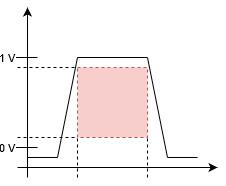
\includegraphics[width=0.4\textwidth]{dvw}
    \centering
    \caption{A Data Validation Window}
    \label{fig:dvw}
\end{figure}

\subsection{Egyéb korlátok}
Megjelentek a párhuzamosság (ILP) hatékonysági korlátai.

\section{A disszipáció csökkentése}
A DVFS (Dynamic Voltage and Frequency Scaling) a dinamikus feszültség és frekvencia szabályozást jelenti (skálázás).
Ez menet közben meghatározza, hogy az adott feladathoz milyen teljesítményre van szükség, majd ehhez igazítja a processzor feszültségét és frekvenciáját.
Példa ilyenre, amikor a mobiltelefon lekapcsolt képernyővel készenléti módban van, majd felvesszük és játszani kezdünk rajta.
Működése:
\begin{enumerate}
    \item szükséges teljesítmény meghatározása
    \item frekvencia hozzáillesztése a szükséges teljesítményhez
    \item órafrekvencia fenntartásához szükséges minimális feszültség beállítása
    \item később kiegészült az AVS-el (Adaptive Voltage Scaling), ez a következő félév anyaga
\end{enumerate}

\section{Az Intel Pentium 4}
A Pentium 4-es CPU 2000-től 2008-ig volt kapható, de a fejlesztését már 2004-ben befejezték, amikor a frekvenciát már nem tudták tovább növelni a statikus disszipáció növekedése miatt.
Kevésbé volt hatékony, mint a korabeli AMD CPU-k, viszont a magasabb órajel miatt nagyobb teljesítményre volt képes.
Míg a Pentium III órajele 500 és 1333 MHz között volt, a P4 1.5 GHz-ről indult és a Prescott architektúrára (2004) elérték a 3.2 GHz-et.

\subsection{Thermal Monitor}
A magasabb frekvenciát a versenytársakéhoz képest jobb hővédelemmel sikerült elérni, ez volt a Thermal Monitor.
Ez egy órajel moduláción alapuló megoldás, ha az érzékelő túlmelegedést észlelt, lekapcsolta (későbbiekben csökkentette) az órajelet.

\subsection{Multimédia}
A P3-hoz képest fejlesztették a multimédiás feldolgozást, 144 új utasítás került be az SSE (FX) és MMX (FP) utasításkészletekbe.

\subsection{Felépítés}
A processzor működési vázlata a \ref{fig:p4}. ábrán látható.
\begin{figure}[H]
    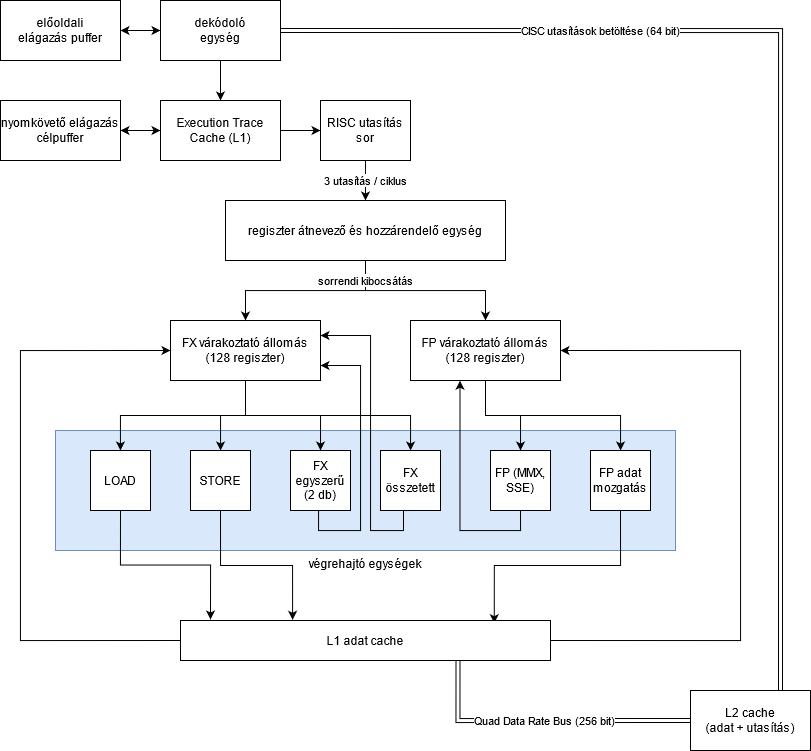
\includegraphics[width=\textwidth]{p4}
    \centering
    \caption{A Pentium 4 processzor működési vázlata}
    \label{fig:p4}
\end{figure}
% 9. előadás vége

\chapter{Szál szinten párhuzamos architektúrák}

\section{Bevezetés}
Az Intel 80386-os processzora óta bevezetett újítások a fogyasztás és a lapkaméret növekedésével jártak, viszont ehhez képest a teljesítmény csak kisebb mértékben javult.
Tehát a teljesítmény növekedése nem állt egyenes arányban a komplexitás növekedésével.
Ez elsősorban az egy magos processzorokra igaz.
Következmény, hogy egyre több tranzisztor kell és nő a fogyasztás.
Ennek megoldásához el kellett térni a klasszikus tervezési elvektől, ahol csak utasítás szinten használták ki a párhuzamosságokat.
A fejlődés következő lépcsőjét a szál szintű párhuzamosság kihasználása jelentette.

\section{A szál}
A szál a program legkisebb önállóan végrehajtható része $\rightarrow$ párhuzamosan futtatható.
Míg az utasítás szintű párhuzamosság felderítésére önmagában képes a hardver, a szálak kihasználásához az operációs rendszer támogatására is szükség van.
% 11. előadás

\chapter{Folyamat szinten párhuzamos architektúrák}

\section{Bevezetés}
A folyamat szinten párhuzamos architektúrák MIMD típusúak, multiprocesszoros rendszerek.

\section{Fejlesztési motivációk}
A multiprocesszoros, folyamat szinten párhuzamos rendszerek kifejlesztését az alábbi tényezők tették szükségessé:
\begin{itemize}
    \item Utasítás szintű párhuzamosság korlátozott lehetőségei:
    \begin{itemize}
        \item Branch prediction soha nem 100\%-os.
        \item Általános célú alkalmazásoknál a programokban lévő utasítás szintű párhuzamosság sokszor ahhoz sem elegendő, hogy 4-6 független végrehajtó egységet ellásson utasításokkal.
    \end{itemize}
    \item Energiahatékonyság: egyes CPU-knál kb. 10-15\% számítási teljesítmény növekedéshez akár 50\% fogyasztás emelkedés is szükséges lehet. Következmény, hogy hatékonyabb lehet n darab CPU-t használni egységnyi órajelen, mint 1 darab CPU-t n-szeres órajelen (jól párhuzamosítható feladatok esetén).
    \item Költséghatékonyság: n darab olcsóbb és lassabb CPU összekapcsolása hatékonyabb lehet, mint 1 darab gyors és drága processzor.
    \item Egyszerű bővíthetőség: ha megfelelően fel van készítve, a bővítése könnyebb lehet egy multiprocesszoros rendszernek.
    \item Hibatűrés: ha az egyik processzor meghibásodik, a többi átveszi a feladatait.
\end{itemize}

\section{Csoportosítás}
\subsection{Memória használat szerint}
\begin{itemize}
    \item Közös memória használatú: van olyan, minden CPU számára látható közös memória, melyen keresztül a folyamatok kommunikálni tudnak egymással.
    \item Elosztott memória használatú: a folyamatok üzenetek segítségével kommunikálnak egymással. Ezek az üzenetküldésen alapuló multiprocesszoros rendszerek.
\end{itemize}
\subsection{Memória elérés ideje szerint}
\begin{itemize}
    \item UMA (Uniform Memory Access): a memória elérés ideje azonos minden CPU számára. Következmény, hogy nincs jelentősége annak, hogy a memóriában hova írjuk az adatot.
    \item NUMA (Non-Uniform Memory Access): a memória műveletek ideje nem azonos. Ezeknél a rendszereknél fontos, hogy egy adat az őt író és az őt olvasó CPU-hoz is közel legyen.
\end{itemize}

\section{Korlátok}
\begin{itemize}
    \item Szoftver: vezérlés áramlásos rendszerekben a párhuzamosságok felderítését szoftveresen kell megoldani. Megoldás:
    \begin{itemize}
        \item olyan compilert írunk, ami képes felfedezni a szoftverek párhuzamosítható részeit és ennek megfelelő kódot generál, vagy
        \item a párhuzamosítást a programozóra bízzuk (főleg ez a működőképesebb).
    \end{itemize}
\end{itemize}

\section{Amdahl törvénye}
Annak eldöntéséhez, hogy érdemes-e folyamat szintű párhuzamosítást alkalmazni, felhasználhatjuk Amdahl törvényét.
Segítségével kiszámolható, hogy az n darab CPU-ból álló rendszer mekkora teljesítmény növekedést tud nyújtani.
Ehhez fontos tudni, hogy milyen mértékben párhuzamosíthatók a folyamatok.
Egy valós program tartalmaz szekvenciális és párhuzamosan futtatható részeket is, ezek alapján pedig feltételezhetjük, hogy egy program P-ed része párhuzamosítható.
Ebből következik, hogy 1-P rész szekvenciálisan futtatható.
Legyen a futási idő 1 darab CPU-n 1 egység.
Ekkor N db CPU esetén a futási idő ideális körülmények között:
\begin{center}
    $(1-P)+\dfrac{P}{N}$ .
\end{center}
Ebből a teljesítmény növekedés:
\begin{center}
    $S\textsubscript{p}(N)=\dfrac{1}{1-P+\dfrac{P}{N}}$ .
\end{center}
Például, ha azt szeretnénk, hogy egy 100 processzoros rendszeren 50-szeres teljesítmény növekedést kapjunk az 1 CPU-hoz képest, akkor
\begin{center}
    $P=\dfrac{S\textsubscript{p}(N)-1}{S\textsubscript{p}(N)}\cdot\dfrac{N}{N-1}\approx0.9898$ ,
\end{center}
tehát a programunk majdnem 100\%-ának párhuzamosíthatónak kell lennie.
Amdahl törvényéből következik, hogy a gyorsulásnak véges határértéke lesz végtelen processzor esetén is, mivel
\begin{center}
    $\displaystyle{\lim_{N \to \infty}}S\textsubscript{p}(N)=\dfrac{1}{1-P}$ ,
\end{center}
így például egy 95\%-ban párhuzamosítható programmal legfeljebb 20-szoros gyorsulás érhető el.
Következmény: a processzorok számát nem gazdaságos egy bizonyos határon túl emelni.

\section{UMA rendszerek}
\subsection{Felépítés}
Az UMA, vagy más néven SMP (Symmetric Multiprocessing) rendszereknél a processzorok egy közös buszon keresztül érik el a memóriát (\ref{fig:uma}. ábra).
Probléma, hogy a közös buszrendszeren keresztül továbbítódik minden adat, így az szűk keresztmetszetet képez.
Ezért a megoldás nem jól skálázható, kb. 8-16 CPU köthető össze a buszrendszer túlterhelése nélkül.
\begin{figure}[H]
    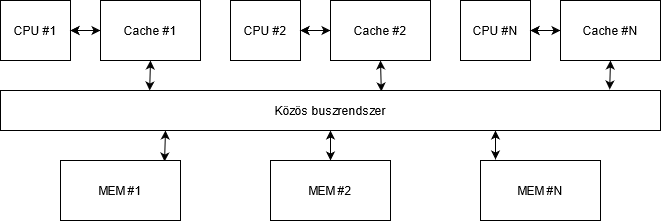
\includegraphics[width=\textwidth]{uma}
    \centering
    \caption{Az UMA rendszerek memória elérése}
    \label{fig:uma}
\end{figure}
\subsection{Gyakorlati példa}
A kezdeti többmagos architektúráknál alkalmazott FSB (Front Side Bus) felépítés UMA elven működik (\ref{fig:fsb}. ábra).
\begin{figure}[H]
    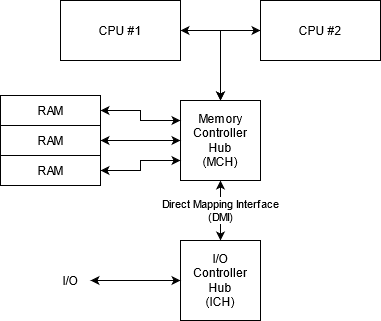
\includegraphics[width=0.6\textwidth]{fsb}
    \centering
    \caption{A tradícionális FSB rendszer felépítése}
    \label{fig:fsb}
\end{figure}

\section{NUMA rendszerek}
\subsection{Felépítés}
Az UMA rendszerek problémáinak kiküszöbölésére fejlesztették a NUMA architektúrákat, amik közös, de tartományokra bontott memória címtérrel rendelkeztek (\ref{fig:numa}. ábra).
A tartományok megfelelői az ábrán a csomópontok.
Eredmény, hogy a buszrendszerre kisebb terhelés esik, így a megoldás jól skálázható.
\begin{figure}[H]
    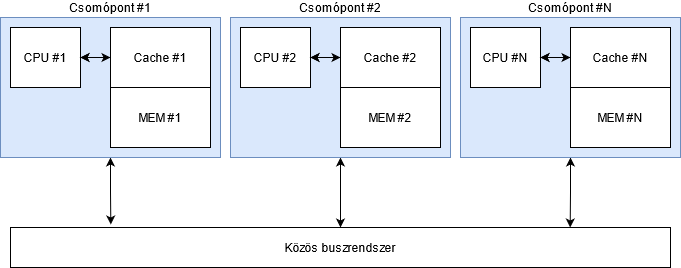
\includegraphics[width=\textwidth]{numa}
    \centering
    \caption{A NUMA rendszerek memória elérése}
    \label{fig:numa}
\end{figure}
\subsection{Csoportosítás}
A NUMA rendszereket két csoportra oszthatjuk:
\begin{itemize}
    \item CC NUMA: cache coherent
    \item NC NUMA: non cache coherent
\end{itemize}

\subsection{Cache coherent}
A cache koherens rendszereknél az adatok legfrissebb példányát a gyorsítótárakban nyilvántartják és frissítik.
Ez a gyakorlatban azt jelenti, hogy ha két CPU ugyanazzal az adattal dolgozna, és mindkettő betölti a gyorsítótárába, majd az egyik módosítja az adatot, a másik CPU gyorsítótárában lévő adatot invalidálja egy figyelő rendszer és az adat frissítésre kerül.
A módszer hátránya, hogy ez komoly adminisztrációt igényel, ami a buszrendszert terheli.
A CC NUMA rendszereket ezért szokás hívni az UMA rendszerek skálázható kiterjesztésének is.
Ez a megoldás kb. 32 CPU-ig skálázható, viszont az UMA-hoz képest a memória műveletek késleltetése 2-7-szeresére növekszik.

\subsection{Non cache coherent}
A nem cache koherens rendszerek nem garantálják, hogy a proceszor mindig az adat legfrissebb verziójával dolgozik, az ebből adódó problémás helyzeteket szoftveresen kell detektálni és kezelni.
Ez a legjobban skálázható megoldás, tervezése és építése könnyű, viszont a programozása sokkal nehezebb.
Általában sok gépes (több összekapcsolt szerver) rendszerekben használják.
Ilyen processzor például az Intel Xeon és az AMD Opteron.

\subsection{Gyakorlati példák}
\subsubsection{Quick Path Interconnect}
A modern többmagos processzorokban a klasszikus FSB felépítés helyett a QPI (Quick Path Interconnect) technológiát használják, ahol a CPU-k egy nagy sebességű buszon (QPI) kommunikálnak egymással (\ref{fig:qpi}. ábra).
Ennek előnye, hogy a memória kontrollerek a processzorok lapkáira vannak integrálva, így a memória elérése gyorsul.
Mivel így már a CPU-knak külön memóriaterületet kell kezelniük, ez egy NUMA architektúrának számít.
\begin{figure}[H]
    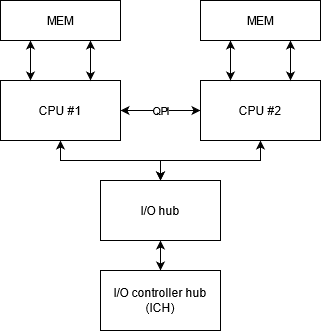
\includegraphics[width=0.5\textwidth]{qpi}
    \centering
    \caption{A Quick Path Interconnect felépítése}
    \label{fig:qpi}
\end{figure}
\subsubsection{Intel Core i}
A mai Core i architektúráknál már a processzorokon belüli magok is eltérő memória területeket kezelnek.
Egy 4 magos CPU-nál két-két mag kap egy közös memóriavezérlőt, a magok pedig egy, a QPI-hez hasonló buszrendszeren kommunikálnak.
A gyors adatelérés érdekében a magok közös L3 cache-t használnak (\ref{fig:corei}. ábra).
\begin{figure}[H]
    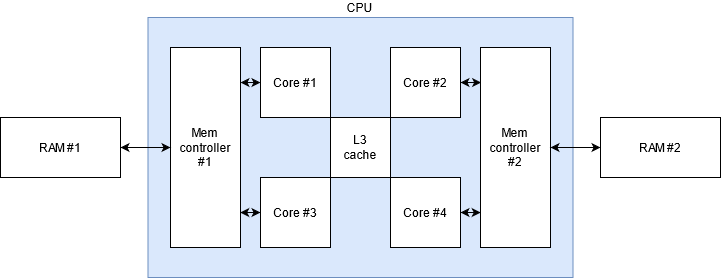
\includegraphics[width=\textwidth]{corei}
    \centering
    \caption{A modern Intel Core i processzorok felépítése}
    \label{fig:corei}
\end{figure}

\section{Összegzés}
A modern több magos és több processzoros rendszerekben inkább NUMA felépítést alkalmaznak.
Az előbb bemutatott Core i processzor is egy példa arra, hogy a nagy, több gépes rendszereken kívül a mikroarchitektúrák szintjén is megtalálhatók a NUMA jellemzők.
A szerverekben cache koherens NUMA rendszerek dominálnak, a nem cache koherens technológiákkal pedig több gépből álló rendszerek építhetők.
% Kilencedik és tizedik előadás

\chapter{Mobil processzorok architektúrája}

\section{Bevezetés}
A modern processzorok sok különálló egységet tartalmaznak, ezek közül a CPU-val foglalkozunk.
Mobil processzorok alatt a mobiltelefonok és a táblagépek processzorait értjük.

Csak kevés gyártó tervez mobil processzorokat és a legtöbbjük nem rendelkezik gyártási kapacitással, kivéve a Samsungot.
A többi gyártó processzorait jellemzően a TSMC vagy a Samsung gyártja le.

A mobil processzorok többsége ARM alapú, de léteznek x86 alapú mobil processzorok is.
x86 alapú processzorokkal az Intel és az AMD próbálkozott, sikertelenül (2016-ban meg is szüntették a gyártást).

\section{ARM licenszek}
Az ARM processzorok gyártóinak két lehetősége van:
\begin{itemize}
    \item Cortex licensz felhasználása
    \item Architektúra licensz felhasználása
\end{itemize}

Cortex licensz esetén a vásárló egy komplett mikroarchitektúra tervet kap meg, konfigurálható opciókkal.
Az architektúra licensz viszont csak arra jogosítja fel a vásárlót, hogy az utasításkészletet használja.

\section{Az ARM alapú mobil processzorok fejlődése}
Az ARM ISA fejlődésével együtt az ARM mobil processzorok is fejlődtek.
Ennek az egyik fontos állomása volt a v7-ről v8-ra átállás, ami behozta a 64 bites támogatást.
Az áttérés során a cégek előtt két út állt:
\begin{itemize}
    \item egyesek megtartották a hagyományos szimmetrikus többmagos felépítést
    \item mások egyúttal áttértek a big.LITTLE architektúrára is
\end{itemize}
Az Apple és a MediaTek szimmetrikus megvalósítást alkalmazott, a Samsung és a Huawei pedig big.LITTLE architektúrát kezdett használni.
A 64 bites áttérés tehát nagyjából egyszerre történt a big.LITTLE átállással, 2013 és 2016 között.

Nem sokkal ezután történt az átállás az ARMv8.2-re (2018), ami a dinamikus magklaszterek használatával jelentős teljesítmény növekedést ereményezett.
Ezzel egyidőben jelentek meg az ARM szerverprocesszorok is.

\section{Az Intel Atom és az AMD Cat család}
Az Intel és AMD hagyományos processzorai a nagy fogyasztás miatt nem voltak alkalmasak a mobil felhasználásra, ezért az Intel 2008-ban, az AMD pedig 2011-ben új processzorokkal állt elő.
Az AMD piacra lépése nagyon későinek számított.

Az Intel Atom processzora a hagyományos processzorokkal ellentétben 2 és 3 széles volt, ennek oka az alacsonyabb fogyasztás.

Ezek ellenére egyik cég se tudott érdemben betörni a mobil piacra, ezért 2015-ben befejezték ezeket a fejlesztéseket.

\section{Windows táblagépekre fejlesztett Core 2 processzorok}
2013-tól a Microsoft megjelent a Surface táblagépekekkel, amik 2 az 1-ben gépek voltak.
Intel processzorokkal szerelték őket, először 2, aztán 4 maggal.
A táblagépek között nagyjából 10\%-os részesedést értek el.

Az elmúlt néhány évben a Windows tabletek is megjelentek Qualcomm ARM processzorokkal.
A céljuk olyan 2 az 1-ben gépek megalkotása, amik nagyon hosszú üzemidővel rendelkeznek (Always on, always connected).
Fő problémájuk a szoftver kompatibilitás.

\section{ARM processzorok az Apple Mac eszközeiben}
Az Apple 2006-tól az Inteltől vásárolta a processzorait.
2020-ban viszont bejelentették, hogy saját processzort fog fejleszteni a MacOS alá.
Az új processzor, az Apple M1 jó teljesítménnyel rendelkezik.

\section{Mobil processzor architektúrák fejlődése}
A fejlődésnél négy fő szakaszt különböztetünk meg:
\begin{itemize}
    \item egymagos processzorok
    \item szimmetrikus többmagos processzorok
    \item big.LITTLE processzorok
    \item DynamIQ klaszter alapú processzorok
\end{itemize}

Az egymagos processzorok használata kb. 2003-tól 2010-ig tartott, általában 32 bitesek voltak.
A többmagos processzoroknál először szimmetrikus felépítést alkalmaztak, 2011-2013-ban, amik szintén 32 bitesek voltak.
A big.LITTLE architektúra 2013-2016-ig tartott, itt megtörtén a 64 bites átállás.
DynamIQ processzorokat 2018-tól gyártanak.

Az egymagos processzorokat nem tárgyaljuk.

\subsection{Szimmetrikus többmagos processzorok}
A desktop processzorok többmagossá válása után kb. 6 évvel, 2011-ben jelentek meg a mobiloknál is a többmagos felépítések.
Cél a teljesítmény növelése.
Az egyik első ilyen rendszer a Samsung Exynos 4412 volt.
\begin{figure}[H]
    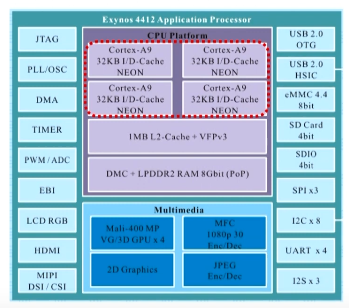
\includegraphics[width=0.8\textwidth]{exynos}
    \centering
    \caption{A Samsung Exynos 4412 felépítése}
    \label{fig:exynos}
\end{figure}
A szimmetrikus többmagos processzorok fő fejlesztési iránya a magok számának növelése volt, a kezdeti 2-ről 4-re, majd 8-ra emelkedett.

Az általános felépítés kettő vagy négy magos magklasztereket jelentett, a klaszteren belül egy közös L2 cache-el.
8 magos rendszereket 2x4 magos klaszterrel készítettek.

\subsection{big.LITTLE architektúrák}
A kifejesztésük fő motivációja a fogyasztás csökkentése.
Az ötlet onnan eredt, hogy az okostelefon használata során nagyon gyakran változik a teljesítmény igény.
Ezért kétféle magot hoztak létre, kis fogyasztású, kis teljesítményűt és nagyobb fogyasztású de nagyobb teljesítményűt.

\subsubsection{Feladatok elosztása}
Az így létrejövő heterogén többmagos rendszerekben a feladatokat többféle módon is fel lehet osztani a magok között:
\begin{itemize}
    \item mester-szolga elv
    \item feladattovábbítás a dedikált végrehajtók felé
    \item más típusú processzor felhasználása
\end{itemize} 

A mester-szolga elvnél van egy megkülönböztetett mester mag és egy vagy több szolga mag.
Ekkor a mester mag látja el a feladatok kiosztását is.
Az IBM, Sony és a Toshiba próbálkozott ilyen elvű processzorral (Cell processzor), de a bonyolult programozás miatt nem volt túl működőképes.

A második esetben a processzorban dedikált végrehajtóegységek vannak, mint pl. GPU.
Minden utasítás ahhoz az egységhez kerül, ami a legalkalmasabb a végrehajtására.

Az utolsó működést tipikusan big.LITTLE architektúráknál használják, ekkor különböző típusú CPU-k működnek együtt.

\subsubsection{big.LITTLE alapelvek}
A big.LITTLE processzorokban kettő vagy több magklaszter dolgozik, amik architekturálisan megegyező magokat tartalmaznak.
A magklaszterek cache koherens módon vannak összekötve.
Ehhez kell egy szoftver, ami a klasztereket vezérli.

\subsubsection{Működési elv}
A big.LITTLE technológia különböző módokon implementálható, mi az exkluzív klaszter kapcsolást vizsgáljuk a működési elv leírásánál.
Feltételezzük még, hogy egy klaszter minden magja azonos munkaponton dolgozik.
\begin{itemize}
    \item egy kernel rutin figyeli a teljesítmény igényt és kiválasztja a megfelelő munkapontot
    \item ha a teljesítmény igény kicsi, a kis klaszter van használatban
    \item ha a teljesítmény igény megnő, klaszter átkapcsolás történik a nagy magokra
    \item ha újra elég a kisebb teljesítmény, a klaszter visszavált a kis magokra
\end{itemize}
Egyszerre csak egy klaszter működhet, ezért ez az exkluzív klaszter kapcsolási rendszer.

\subsubsection{Megvalósítás}
A technológia hardverkövetleményei:
\begin{itemize}
    \item a kis és nagy klasztereknek architektúrálisan azonosnak kell lennie
    \item a gyors átkapcsoláshoz szükséges egy cache koherens megoldás
    \item a megengedett magszám klaszterenként általában 4
    \item megfelelő szoftvertámogatás szükséges, amit a processzorgyártó ad át a gyártóknak, kernel kiegészítések formájában
\end{itemize}

A big.LITTLE architektúrákat három szempont szerint viszgáljuk:
\begin{itemize}
    \item klaszterek és magok száma
    \item ütemezési megoldások
    \item feszültség és frekvencia ellátás
\end{itemize}

Mag klaszterek szerint két vagy három klaszteres rendszereket különböztetünk meg.
Az egyes klaszterekben 1, 2, 3 vagy 4 mag lehet.

Az ütemezési megoldások vizsgálatánál egy 2 klaszteres processzort tekintünk.
Az ütemező működhet klaszter vagy mag alapon.
Mindkét esetben kétfajta implemtáció lehet: exkluzív és inkluzív.
Exkluzívnál vagy egyik, vagy másik klaszter van hozzárendelve egy adott feladathoz.
Inkluzívnál megengedett, hogy a két klaszter egyszerre működjön nagy teljesítmény igény esetén.
Általában exkluzív implementációt használnak, mivel az inkluzívat nehezebb implementálni és viszonylag kis gyorsulást eredményez.

A mag alapú ütemezés is történhet exkluzív vagy inkluzív módon.
Exkluzív mag allokációnál a magokat kis-nagy párokba szervezik.
Az ütemező a terheléstől függően a nagy vagy kis magot választja ki.
Inkluzívnál viszont minden mag külön-külön aktiválható, ezért ez egy globális ütemező.
Ma ez a legelterjedtebb.

A felhasználói igény döntően a frekvenciát dönti el, ami meghatározza a szükséges feszültséget.
A szabályzás üzemeltethet minden magot azonos feszültségen és frekvencián, szabályozhatja magonként a frekvenciát, közös feszültséget tartva, vagy magonként különböző frekvencia és feszültség beállításokat alkalmazhat.
A leghatékonyabb az utolsó megoldás.

\subsection{DynamIQ magklaszterek}
Az ARM 2013-ban kezdte el fejleszteni a technológiát, 2018-ban kezdték használni.
Ez jelenti a big.LITTLE architektúrák utáni lépcsőfokát a fejlődésnek.

A dinamikus magklaszter két különböző magot képes tartalmazni: kis mag és nagy mag.
Különbség a big.LITTLE klaszterekhez képest, hogy a magokat közel tetszőlegesen lehet párosítani.

\subsubsection{Energy Aware Scheduling}
A fogyasztást egy intelligens fogyasztáscsökkentő eljárás bevezetésével javította, ez az EAS - Energy Aware Scheduling.
Ez előtt a Linux kernel a CFS-t, azaz a Completely Fair Schedulert használta, ami elsőrorban teljesítményre optimalizált.
Hátránya, hogy heterogén rendszerekben nem működik elég hatékonyan.
Az EAS ezzel szemben figyelembe veszi a big.LITTLE felépítést, így elérve a lehető legalacsonyabb fogyasztást.

\subsubsection{DynamIQ klaszterek jellemzői}
\begin{itemize}
    \item ARMv8.2-t támogatnak
    \item két típusú magot tartalmazhatnak a klaszterek
    \item magonkénti L2 cache-el rendelkezik - ez lényegesen jobb megoldás, mint a közös L2 cache
    \item megjelenik a harmadik szintű gyorsítótár, a magok közös L3 cache-el rendelkeznek
    \item a klaszter egy új egységet is tartalmaz, ez a DSU (Dynamic Shared Unit): ebben van az L3 cache és egy snoop filter, ami a cache koherencia fenntartását teszi hatékonyabbá. Következmény, hogy alacsonyabb késleltetéssel érhetők el a gyorsítótárak.
    \item a magok partícionálhatók: négy partíció hozható létre, amik magokat, külső gyorsítókat és az L3 cache bizonyos részeit tartalmazzák. A partíciókat feladatok szerint lehet kialakítani.
    \item finomabb feszültség-frekvencia szabályozás, a különböző partíciók eltérő frekvencián és feszültségen működhetnek
\end{itemize}

\section{Magok szélességének fejlődése}
A processzormagok két részre bonthatók: frontend és backend.
A frontend több utasítást dolgoz fel szekvenciálisan és küldi ki a backend számára.
A backendben egyedi utasítások kerülnek feldolgozásra a megfelelő futószalagokon.
A mag szélessége a mag legszűkebb keresztmetszetét jelöli, ami legtöbbször a dekódoló szélességének felel meg.
Teljesítmény szempontjából minél szélesebb egy mag, annál gyorsabb a processzor, a fogyasztás viszont fordítva működik.
Fontos szempont még, hogy a mag tud-e többszálas működést.
A szálak gyorsító hatása az adott felhasználástól függ.

Az első mobil rendszerekben (2000-es évek eleje) 2-3 széles processzorok dolgoztak.
Ez nem sokat változott a 64 bites átállással, mivel a kisebb teljesítményű rendszerek maradtak 2 szélesek, a nagyobb teljesítményűek pedig 3 szélesek.
Ezután az Intel és az AMD megjelentek a saját mobil processzoraikkal, amik 2 szélesek voltak, viszont nem voltak versenyképesek.

Az ARMv8 és v8.2 ISA-ra épülő processzoroknál a magasabb teljesítmény érdekében áttértek 4-es és 5-ös szélességre.
Ennek eredménye, hogy a kibocsátási és a kiküldési ráta is jelentősen megnőtt.
A szélesség növeléséhez növelni kellett az erőforrásokat, így a ROB méretét is.
Ezzel együtt megjelent a MOP cache, ami a már dekódolt utasításokat tudja tárolni és újrahasználni, pl. elágazásbecslés visszatörlésnél vagy ciklusnál.

Az Apple nagyon hamar, az A7 processzorukban (2013) áttért a 6 széles magokra.
Ezzel teljesítményben minden más processzort leelőzött, amit később tartott is.
Később az A11 és A12X processzorokban 7-es, majd az A13, A14 és M1 processzorokban 8-as szélességű magokat alkalmaztak.

A Samsung szintén nagy lépésekkel fejlődött a Mongoose processzorával, 6-os szélességet értek el, a 8 széles processzoruk fejlesztését viszont leállították.

Az AMD hagyományos desktop architektúrái ezzel szemben csak 4 szélességig fejlődtek (Bulldozer család), az Intelek viszont 6-ig (Alder Lake).
Az AMD ezzel sokat veszített a piacból.
Tehát a mobil processzorok szélesebbek a hagyományos rendszerknél.
Ennek oka, hogy a hagyományos rendszerek CISC architektúrák, ahol változó hosszúak az utasítások.
A RISC-ek ezzel szemben fix utasításhosszal rendelkeznek, ezeket pedig sokkal könnyebb dekódolni.

\subsection{A Samsung Mongoose családjának fejlődése}
A Samsung 2010-ben alapított egy processzor fejlesztő központot Austinban, ahol a Mongoose családot fejlesztették.
Első megjelent processzoruk volt az ARMv8 alapú M1, 2016-ban.
Később áttértek az ARMv8.2-re, majd az M6-al leálltak a fejlesztéssel.
Az elkészült processzorokat a Samsung Galaxy telefonokban használták.
A több száz alkalmazott mérnök ellenére a Samsung 2019-ben bezárta a központot, utána pedig publikálták a processzorok fejlődését.

Az első Mongoose processzor a Galaxy S7-ben jelent meg, az utolsó pedig a Galaxy S20-ban (2020).
Kiemelt ezek közül az M3-as mag, amivel a Samsung áttért az ARMv8-ra.
A 10 éves fejlesztés során a teljesítmény növelését három területen keresték:
\begin{itemize}
    \item kisebb igényű feladatok végrehajtásának gyorsítása: ezen a területen arra jutottak, hogy az előlehívás és a cache koherencia protokollok optimalizálásával lehet gyorsulást elérni
    \item közepes igényű feladatok: itt az elágazás kezelés és a cache fejlesztésével tudtak eredményeket elérni
    \item nagy igényű feladatok: ezeknél főleg a szélesség növelésével és a megfelelő erőforrások biztosításával lehetett gyorsítani
\end{itemize}
Ezeknek a szempontoknak a figyelembevételével az M6 az M1-hez képest 2,71-szer nagyobb IPC-t (Instruction per Cycle) ért el.
Ez évente 20\%-os növekedésnek felel meg.

A teljesítményt a programfutások trace-elésével vizsgálták és ezek alapján állapították meg a fejlesztési lehetőségeket.

\subsubsection{A mikrooperációs cache}
A magok szélességének növelésével szükségessé vált az utasítások gyorsítótárazása, ezért az M5 bevezetta a mikrooperációs cache-t.
Ez 384 utasítást tudott tárolni, a használatával a cache-elt utasításoknál megspórolható a lehívás és a dekódolás.
A többi gyártóhoz képest későn vezették be.

\subsubsection{Végrehajtó egységek száma}
A szélesség duplájára növelésével a végrehajtó egységek is lépést tartottak, itt is kb. kétszeres növekedés ment végbe.

\subsubsection{Összegzés}
A fejlesztések ellenére az ARM processzorok gyorsabban fejlődtek, ezért a Samsung is visszatért ezek használatára és felhagyott a saját fejlesztéseivel.


% Tizenegyedik és tizenkettedik előadás

\chapter{Az Intel 2S szerver processzorai}

\section{Bevezetés}
Az Intel szerver processzorai két csoportra oszthatók:
\begin{itemize}
    \item Xeon - x86 alapúak, 2004-től 64 biten
    \item Itanium - VLIW alapúak
\end{itemize}

A továbbiakban a 64 bites Xeonokat vizsgáljuk.
Az első 64 bites 2S szerver processzor a Nocona volt, ami a Pentium 4-re épült.
A Nocona után már minden szerverprocesszor többmagos volt.

Elnevezések: DP - dual processor, MP - multi processzor.
Később ezeket váltották a 2S, 4S és 8S jelölések, amik a foglalatok számára utalnak.
Csak a 2S szerverekkel foglalkozunk.

\subsection{A szerverprocesszorok piaca}
A szerverek nagyrészt 1S és 2S rendszerekre épülnek (91\%).

2005 környéként két jelentős típusú szerver volt forgalomban:
\begin{itemize}
    \item a SUN által képviselt RISC rendszerek
    \item az Intel x86 alapú szerverei
\end{itemize}
Napjainkban gyakorlatilag csak x86 alapú szervereket használunk.

Az Intel és az AMD versenye az évek során:
\begin{figure}[H]
    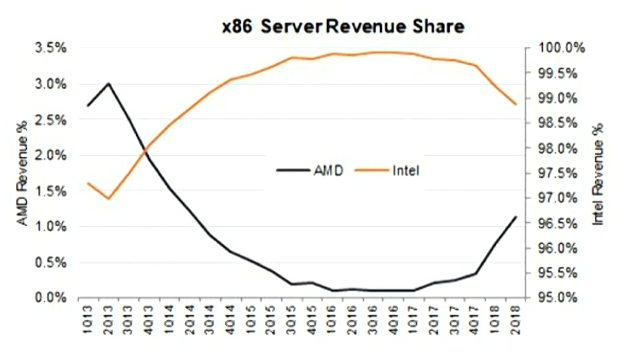
\includegraphics[width=0.8\textwidth]{intelamd}
    \centering
    \caption{Intel és AMD szerver eladások}
    \label{fig:intelamd}
\end{figure}
Az AMD a Zen processzorokkal tudott újra nagyobb részesedést szerezni.
Újdonság, hogy az ARM is bejelentett egy új, szerverorientált családot, a Neoverse-t.
Várható, hogy az ARM processzorok valós konkurenciát fognak jelenteni az AMD-nek és Intelnek.

\subsection{A platform fogalma és a kompatibilitás}
Platformnak tekintjük a rendszer fő komponenseit (a vázát).
Ezek a komponensek:
\begin{itemize}
    \item processzor
    \item chipset
    \item interfészek
\end{itemize}

Egy processzor tehát akkor kompatibilis egy platformmal, ha az adott interfészt támogatja.

\subsection{Szerverplatformok osztályozása}
A platformokat többféleképpen osztályozhatjuk:
\begin{itemize}
    \item foglalatok száma
    \item memória csatolási felület
    \item teljesítmény osztály
    \item lapkakészlet chipeinek száma
\end{itemize}

\subsubsection{Foglalatok száma szerint}
\begin{itemize}
    \item egyprocesszoros
    \item többprocesszoros (2S, 4S, 8S, 8-nál több processzoros)
\end{itemize}

\subsubsection{Az Intel Optane memória}
Az Optane memória egy nem felejtő (non-volatile) memória, ami a memória méretét terjeszti ki, az ezen tárolt adatokat pedig nem kell háttértárra menteni.
Ez egy teljesen új memória technológiát alkalmaz, ez a 3D XPoint, ami a kristályszerkezek különböző állapotait használja ki.

\subsubsection{Memória csatlakozás szerint}
\begin{itemize}
    \item UMA (Uniform Memory Access): azonos elérési időt biztosít minden magnak és processzornak, mivel a memória a memória vezérlő chipre kapcsolódik
    \item NUMA (Non-Uniform Memory Access): a memória a processzorhoz van illesztve, ekkor a processzorok között eltér a memória különböző területeinek az elérése
\end{itemize}
Mindkét esetben minden processzor eléri a teljes memóriaterületet.
NUMA esetében egy adott processzorhoz tartozik lokális (közvetlenül csatlakozó) és távoli memória is.
Távoli memória esetén az elérés egy másik processzorok keresztül történik.

Napjainkban a NUMA technológia dominál.

\subsubsection{Teljesítmény kategória szerint}
Három nagy csoport különböztethető meg:
\begin{itemize}
    \item mainstream
    \item nagyobb teljesítményű
    \item kisebb teljesítményű
\end{itemize}
Az első szerver processzoroknál még nem voltak külön kategóriák, ezeket tekintjük mainstreamnek.

\subsubsection{Chipkészlet chipeinek száma szerint}
\begin{itemize}
    \item két chipet tartalmazó chipkészlet (északi és déli híd)
    \item egy chipes rendszer (a memória és PCI vezérlő a processzorra költözött)
\end{itemize}

\section{Elnevezési rendszerek}
2005-ig az Intel egyszerű elnevezéseket alkalmaztak, a frekvencia és a típus szerint nevezte el a processzorait pl. Intel Xeon 2.8 GHz DP.
Az AMD ekkor a processzorait az alapján nevezte el, hogy az előző generációhoz képest milyen gyorsulást ért el, pl. AMD Athlon 1600+.

Később az Intel áttért az AMD-hez hasonló nevezékekre, a relatív teljesítmény alapján megjelentek a 3000-es, 5000-es, 7000-es és 9000-es processzorok.
A probléma ezzekkel a nevekkel, hogy nem sokat mondanak el a teljesítményről, ezért ezután az EX (Expandable, nagy teljesítményű), EP (Efficient performance, mainstream) és az EN (Entry level, belépőszint) jelölésekkel látta el a processzorait.
2011-ben egy részletesebb elnevezési sémát vezetett be az Intel.

Erre egy példa: Intel Xeon E7-4820 v2.
Az E(3/5/7) a termékcsaládot jelenti, összhangban a desktopok i3, i5, i7 rendszereivel.
A példában a 4-es szám megadja, hogy hány processzort támogat a rendszer.
A 8-as szám a socket típust jelöli, ami valójában a teljesítmény kategóriának felel meg (4=EN, 6=EP vagy 8=EX).
A 2-es a processzor SKU-ját (Storage Keeping Unit) jelenti, ami gyakorlatilag a modellszám.
Végül a v2 a verziószám, a Sandy Bridge volt az első verzió, ezt még nem jelölték külön.
A v2 tehát egy Ivy Bridge processzor.
Ezek közben az Itanium elnevezése nem változott.

Az EX, EP és EN platformok több szempontból is eltérnek egymástól:
\begin{itemize}
    \item memória csatolás módja
    \item rendszer linkek száma
    \item memória csatornák száma
    \item PCIe vonalpárok száma
\end{itemize}

Az Intel legújabb elnevezési rendszere a Skylake családdal mutatkozott be, 2017-ben.
Az új processzorcsalád egy skálázható koncepciót követ:
\begin{itemize}
    \item egységesíti a processzorok felépítését a támogatott foglalatok számától függetlenül
    \item négy teljesítmény kategóriát vezet be az E5 és E7 helyett, az E3-at pedig megszüntetik
\end{itemize}
Az új teljesítmény kategóriák:
\begin{itemize}
    \item Platinum
    \item Gold
    \item Silver
    \item Bronze
\end{itemize}
A különböző osztályok különböző mennyiségű processzort támogatnak.
Az új 4 számjegyű jelölési rendszer pedig a következő ábrán látható.
\begin{figure}[H]
    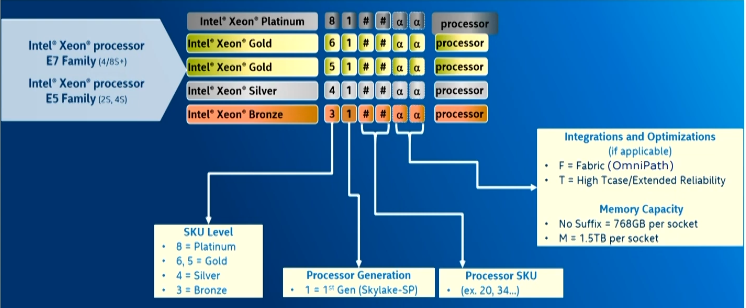
\includegraphics[width=0.8\textwidth]{naming}
    \centering
    \caption{Az Intel legújabb szerver processzor nevezéktana}
    \label{fig:naming}
\end{figure}

\section{Processzorok fejlődése}
Az első Intel 64 bites szerver processzor még egy magos volt (Nocona).
A fejlődés során három fő fázis különböztethető meg:
\begin{itemize}
    \item dedikált szerver processzorok 2S és 4S konfigurációkhoz (2004-2007)
    \item piaci szegmens specifikus processzorok (EN, EP, EX), ezek már mind NUMA processzorok (2010-2016)
    \item skálázható szerver platformok (2017-)
\end{itemize}

A fejlődést négy szempont szerint vizsgálhatjuk:
\begin{itemize}
    \item memóriacsatlakozás (UMA, NUMA)
    \item platform kialakítás (dedikált, szegmens orientált, skálázható)
    \item teljesítmény kategória
    \item támogatott processzorok száma 
\end{itemize}
Először az UMA rendszerek jelentek meg, amik 2 vagy 4 processzort támogattak és dedikált platformnak számítottak.
Következő lépcsőben NUMA rendszerekről beszélhetünk, amik szegmens orientáltak voltak és 3 különböző teljesítmény osztályban készültek, legfeljebb 8 támogatott processzorral
Végül a skálázható platformok jelentek meg, de az Intel közben bejelentett két dedikált processzort.

\section{A memória alrendszerek tervezési kihívásai}
A szerver processzorok fejlődésének első fázisában a magok száma körülbelül két évente duplázódott.
Ez összhangban volt Moore törvényével.
A folyamat akkor változott meg, amikor az L3 cache-ek megjelentek, amik nagyon nagy részét lefoglalták a tranzisztoroknak.
Következmény, hogy a magok számának duplázódása lelassult, már nagyjából 4 év kellett hozzá.
Itt már eltér a fejlődés a Moore szabálytól, mivel a processzor lapka méretét nem tudták arányosan növelni a növekvő gyártási hibaarány miatt (emiatt a hűtés problémásabb volt, a tranzisztorok összezsúfolódtak, a disszipáció korlátozta a tranzisztorok növekedését).
A következő torpanás a 10 nm-es technológia kifejlesztésénél jött, de utána visszatért a 4 évenkénti duplázódás.

A memóriák ezzel szemben 8 évente duplázták a teljesítményüket.
A magszámok tehát sokkal gyorsabban nőttek, mint a memória gyorsasága.
Az egy magra jutó memória sávszélesség viszont meghatározó a rendszer összteljesítményénél, ideális esetben ez a generációk között konstans marad, hogy ne jelentsen szűk keresztmetszetet a memória.
A memóriák sebbessége viszont nem tudta tartani a lépést, ezért a memória csatornák számát kellett növelni az arány fenntartása érdekében.

Megfigyelték, hogy egy adott magszámhoz hány memóriacsatorna szükséges: 2 magnál még elég 2 csatorna, 32 magos rendszerek esetén viszont már 8 csatornára van szükség.
Probléma, hogy a csatornák számának növelése technikailag nagyon nehéz (több vezeték kell, megjelennek az áthallások, stb.).

\section{Skálázható 2S Intel szerver processzorok}
A skálázható szerver processzorok a fejlődés harmadik fázisát jelentik.
Az Intel két skálázható processzorcsaládja a Purley (Skylake, Cascade lake alapok) és a Whitley (Ice lake alapok).
Ezek mind NUMA processzorok.
A Purley Platinum processzorok 1-8, a Goldok 1-4, a Silver és a Bronze osztályú processzorok pedig 1-2 processzort támogatnak.
A Whitley család viszont legfeljebb 2 processzorig skálázható, ezért ez nem is igazán számít skálázhatónak.

A Purley platformot 2017-ben jelentették be, 10 nm technológiával készül.
Fő célja az adatközponti, felhő és mesterséges intelligencia felhasználások támogatása.
Fontos, hogy egységesíti a processzorok tervezését, a 2S, 4S és 8S konfigurációk azonos elemekből építkeznek.

\subsection{Teljesítmény}
A Skylake az Intel kétfázisú fejlesztési ciklusában a Tock fázisba esik, tehát új architektúrát jelent és kb. 10\%-os teljesítmény növekedést hozott.
Ha a 2006-ban megjelent Core 2 szerver processzorokhoz hasonlítjuk a Purley (Skylake) CPU-kat, többszálas teljesítményben kb. 41-szeres növekedést értek el.
A SPECint egyszálas benchmark szerint 3,8-szoros a teljesítmény.
A többszálas végrehajtás nagyon nagy mértékben nőtt a növekvő magszám miatt.

\subsection{Interconnect}
A Broadwell processzorok adatgyűrűs adatkapcsolati megoldással rendelkeznek, ez a megoldás viszont a magszám növekedésével egyre komplexebbé vált, csökkent a hatékonysága.
Ezért a Skylake-nál egy 2D-s adatkapcsolati réteg jelent meg, ahol az adatok csomagokban közlekednek.
Ez a váltás nagyban hozzájárult a rendszer gyorsulásához.

\subsection{A Skylake-et követő architektúrák}
A Skylake-el az Intel áttért egy három fázisú fejlesztési modellre a korábbi tick-tock helyett.
Az első fázisban megtörténik a technológiai váltás (csíkszélesség csökkentése), ezt követi az új mikroarchitektúra, majd ezt követően több lépésben optimalizálják a mikroarchitektúrát.

\subsection{A Cascade Lake szerver processzorok}
A Cascade Lake alapú Purley processzorok a skálázható Skylake CPU-k optimalizálása.
A Cascade Lake-en belül két sorozat létezik: SP és AP.
Míg az SP a hagyományos rendszer, az AP két lapkát integrál egy tokban.

\subsubsection{SP vonal}
Az SP 2019-ben jelent meg, legfeljebb 28 magot támogat.
14++ nm-es technológiával készült, ami a 14 nm-es optimalizált változata.
Sokban nem különbözik az előző rendszerre, viszont tartalmaz több optimalizációt és új neurális kiterjesztéseket vezet be.

Újítás még az Optane memória támogatása és biztonsági javítások.

\subsubsection{AP vonal}
Az AP 2x28, azaz 56 magot alkalmaz, csak a Platinum kategóriás processzorok valósítják meg.
Forrasztandó tokozással érkezik.

Elsősorban nagy számítási igényű alkalmazásokhoz, mesterséges intelligenciához vagy IaaS megoldásokhoz ajánlják.
Csak OEM-ek számára eladó, csak teljes eszköz formájában (számítási modulok).
Méretre kimondottan nagy a processzor, 76x76 mm.

A támogatott memória mennyisége és sebessége is megnőtt a Skylake-hez képest.
Itt is megjelent az Optane memória, az új utasítás kiterjesztés és a biztonsági javítások.

Két ilyen processzor megfelelően összekötve már egy négy processzoros rendszert ad.

\subsection{A Whitley szerver processzorok}
A Whitley a Purley-t követő processzorcsalád.
2021 áprilisában jelent meg, 10 nm-es technológiára épül.

Az Intel skálázható szerver platformként árulja, de a Whitley csak 1 és 2 processzort támogat, a 4-8 processzoros rendszerekhez külön család tartozik, ez a Cedar Island.
Tehát ez nem teljesen skálázható, csak egy szükségmegoldás.
A Purley valódi utódja még nem jelent meg.

\subsubsection{A Whitley (Ice Lake) újításai}
Az előző generáció 6 memóriacsatornája helyett 8-al rendelkezik, ami indokolt is, mivel max. 40 magot támogat a 28 helyett.
Növekedett a ROB mérete, a regiszterfájlok és a cache-ek méretei is.

\subsubsection{Konkurencia}
Az Intel Ice Lake processzorai lemaradtak az AMD és az Altra rendszereitől.

\end{document}